%% Physics of Fluids — Special Issue: Scientific Machine Learning and
%% Physics-Informed AI for Multiscale and Multiphysics Fluid Mechanics
%% Benchmark paper. Content ported/reframed from ../iclr2027/main.tex (post-P1),
%% FLEET_SUMMARY_TABLE_2026-08-30.md, and the kolmogorov2d classical JSONs.
%%
%% Working title candidates (pick one, keep it — the artifact release carries it):
%%   FlowRecon-Bench / SparseFlowBench / RECON-FM Bench
\documentclass[aip,pof,reprint,amsmath,amssymb,superscriptaddress]{revtex4-1}

\usepackage{graphicx}
\usepackage{booktabs}
\usepackage{multirow}
\usepackage{bm}
\usepackage{xcolor}
\usepackage{hyperref}
\newcommand{\todo}[1]{\textcolor{red}{[TODO: #1]}}

% Method-name macros: our model is DMF-Gen, taken as-is from Wang et al.
% (Direct Measurement-to-Field Generation) and cited; no method-novelty claims here.
\newcommand{\dmfgen}{DMF-Gen}
\newcommand{\benchname}{FlowRecon-Bench}

\begin{document}

\title{\benchname{}: A benchmark for sparse-sensor flow-field reconstruction
across flow regimes, with calibrated uncertainty}

\author{Nicolas Tricard}
\affiliation{Department of Mechanical Engineering, Massachusetts Institute of
Technology, Cambridge, Massachusetts 02139, USA}
% \todo{co-authors + affiliations — needs Nick's input at writing time}

\date{\today}

\begin{abstract}
Reconstructing a full flow field from sparse point sensors is a core task of
experimental and operational fluid mechanics, and a rapidly growing machine-learning
literature now addresses it with deterministic operator learners and conditional
generative models. Yet the field has no shared benchmark: published methods are
evaluated on incompatible, often temporally leaky splits, ensembles are drawn but
never scored with proper probabilistic metrics, and classical baselines are rarely
reported. We present \benchname{}, a benchmark spanning three flow regimes ---
laminar cylinder vortex shedding (2D, multi-Reynolds), two-dimensional Kolmogorov
turbulence, and three-dimensional isotropic turbulence (JHTDB) --- evaluated
with leakage-audited splits, frozen sensor manifests, per-channel accuracy, proper scoring rules
(CRPS, coverage, spread--error), physics metrics (windowed spectra, structure
functions), and matched cost accounting (training and inference runtime and peak
memory) for every method. Across a fidelity-audited fleet of twelve-plus methods
--- interpolation and gappy-POD anchors, deterministic operator learners, latent
and ambient generative models including \dmfgen{} --- we find that method ranking
is regime-dependent, and no method wins twice: gappy POD with 20 modes wins
the laminar cylinder outright (0.056 relative $L_2$, including the
never-observed pressure at 0.051), a deterministic operator learner leads
two-dimensional turbulence (Geo-FNO 0.385) while being beaten on CRPS by every
generative model, and latent flow matching, SiT and interpolation split the
channels of 3D turbulence. No method recovers unobserved channels of 3D
turbulence, though gappy POD recovers them on the cylinder; nearly every scored
ensemble is under-dispersed, and post-hoc recalibration partially repairs it. Benchmark
scores are systematically worse than literature-reported numbers on the same
data, and we show by controlled ablation that the gap is evaluation protocol
--- same-trajectory splits, uniform rather than scattered sensing, and
favorable reporting --- rather than model capability. We release the
datasets, splits, sensor manifests, configurations, and evaluation driver as a
versioned artifact. \todo{finalize abstract numbers and artifact DOI}
\end{abstract}

\maketitle

\section{Introduction}\label{sec:intro}

Flow fields govern systems that experiments can only observe pointwise:
particle-image velocimetry resolves planes of a turbulent flow while the
surrounding volume goes unmeasured, flight-test campaigns record surface pressure
at taps while the off-body flow that determines performance is inaccessible, and
environmental monitoring networks sample the atmosphere at stations kilometers
apart. Recovering the full field from such sparse, indirect data is a
long-standing inverse problem,\cite{callaham2019robust,raissi2020hidden,vinuesa2023transformative}
and at realistic sensor densities it is severely ill-posed: many fields fit the
data, and the missing information sits disproportionately at the small scales.
A machine-learning literature now more than a decade deep addresses it with
deterministic reconstruction networks,\cite{fukami2021global,santos2023senseiver,erichson2020shallow,dang2025flronet}
and, more recently, with conditional generative models that sample the
distribution of fields consistent with the observations rather than regressing
to its mean.\cite{shu2023physics,li2024s3gm,huang2024diffusionpde,du2024confild,oommen2026turbulent,zhuang2025spatially}

What that literature does not have is a shared evaluation. Community benchmarks
for scientific machine learning --- PDEBench, The Well, CFDBench, AirfRANS, and
their successors --- pose forward-surrogate or uniform-downsampling
super-resolution tasks, not reconstruction from scattered point sensors; the
Johns Hopkins Turbulence Database is a query service with no canonical protocol,
and published sparse-reconstruction papers each cut their own incompatible
extraction from it. Three consequences follow, and this paper documents all
three. First, \emph{splits leak}: turbulence snapshots are strongly
autocorrelated in time, and the standard random-in-time split makes every test
frame a near-duplicate of a training frame. On our 3D turbulence data,
frame-to-frame correlation is 1.00 at unit separation; under a shuffled split
the strongest latent generative baseline scores 0.14 relative $L_2$, and under
an honest spatially disjoint split the same model scores 0.56 --- a factor of
four, larger than every method-to-method gap we measure
(Sec.~\ref{sec:leakage}). Second, \emph{ensembles are drawn but not scored}:
generative reconstruction papers routinely show mean-and-standard-deviation
maps, several claim calibrated uncertainty on that evidence alone, and, to our
knowledge, none reports a proper scoring rule or a calibration diagnostic for
3D single-snapshot reconstruction from scattered
sensors;\cite{gneiting2007strictly,rybchuk2023ensemble,manshausen2025generative,giral2026genda,gao2026uqshred}
every scored precedent in adjacent settings is under-dispersed. Third,
\emph{classical baselines are absent}: training-free interpolation and gappy
proper-orthogonal-decomposition floors are rarely reported, and we find one of
them (inverse-distance weighting) beats every deep model's observed-channel
error on 3D turbulence at 1\% sensor density. A consequence worth stating
plainly up front: every number and image in this paper will look worse than
its counterparts in the literature, and Sec.~\ref{sec:leakage} shows by
controlled ablation --- same checkpoints, protocols swapped --- that this
gap is the protocol, not the models.

\benchname{} is our response: a benchmark for sparse-sensor flow reconstruction
built to answer the question a practitioner actually has --- \emph{which method
family should I use, in which flow regime, at what sensor budget, with what
uncertainty and at what cost?} It spans three regimes chosen so that each
isolates one axis of difficulty (Sec.~\ref{sec:datasets}): laminar cylinder
vortex shedding, where the dynamics are low-dimensional and classical linear
methods should be near-optimal; two-dimensional Kolmogorov turbulence, the
standard testbed of the 2D generative literature;\cite{shu2023physics,li2024s3gm}
and three-dimensional isotropic turbulence under a spatially disjoint
evaluation protocol. Every method is evaluated under identical seeded sensor draws, identical
augmentation, leakage-controlled splits with a strict tune/test separation,
per-channel accuracy, fair CRPS, coverage and spread--error diagnostics,
windowed spectral metrics, and --- because model selection in practice is a
cost--benefit decision --- measured training and inference runtime and peak
memory for every row.

Our contributions are the benchmark and the findings it forces. (i) A
three-regime task suite with leakage-audited splits, frozen sensor manifests,
and a fingerprinted evaluation driver, released as a versioned artifact
together with per-method configurations and audit notes. (ii) A
fidelity-audited fleet of twelve-plus methods spanning classical anchors,
deterministic operator learners, latent generative and ambient generative
routes, parameter-matched where the published configurations allow and
budget-disclosed where they do not (Sec.~\ref{sec:methods}). (iii) Findings
that generalize beyond any single table: method ranking is regime-dependent;
no method recovers channels the sensors do not observe in 3D turbulence
(a fleet-wide identifiability limit, not a per-method defect); accuracy and
sample realism trade off through the sampler's operating point, so ranking
generative models on mean-field error alone is misleading
(Sec.~\ref{sec:dp}); nearly every scored ensemble is under-dispersed, and a post-hoc
recalibration fitted on a disjoint tuning split repairs stated coverage
(Sec.~\ref{sec:calibration}); and the computational axis separates grid
methods, whose memory walls we measure, from point methods, whose costs are
flat in resolution (Sec.~\ref{sec:cost}).

\section{Benchmark design}\label{sec:design}

\subsection{Task}\label{sec:task}

Let $u:\Omega\to\mathbb{R}^{C}$ be a flow field drawn from a distribution over
fields (snapshots of a turbulent flow, solutions over varying geometry). It is
observed through a measurement operator returning readings
$\mathcal{O}=\{(\bm{x}_j,\,c_j,\,y_j)\}_{j=1}^{M}$ with
$y_j = u_{c_j}(\bm{x}_j)+\varepsilon_j$, where $\bm{x}_j$ is a sensor location,
$c_j$ indexes the observed quantity, and $\varepsilon_j$ is noise. The task is
single-snapshot reconstruction: estimate $u$ --- or, for probabilistic methods,
sample an approximation to $p(u\mid\mathcal{O})$ --- at all query locations,
with no access to sensor time histories, initial conditions, or the governing
solver. This covers sensors scattered arbitrarily or confined to a surface,
observed quantities forming a subset of the target channels, and corrupted
readings. Sequential assimilation and forward surrogacy are deliberately out of
scope; they are different problems with different information budgets.

\subsection{Datasets: three flow regimes}\label{sec:datasets}

Each dataset is chosen to isolate one axis of difficulty
(Table~\ref{tab:regimes}); preprocessing details and download/regeneration
recipes ship with the artifact.

\begin{table*}[tbp]
\caption{\label{tab:regimes}The three regimes of \benchname{}. Each dataset
isolates one axis of difficulty; the split column names the leakage-controlled
protocol (Sec.~\ref{sec:splits}).}
\footnotesize
\begin{ruledtabular}
\begin{tabular}{llllll}
Regime & Dataset & Points & Channels & Split & Axis isolated \\
\hline
Laminar periodic & Cylinder wake (new) & $2.4{\times}10^{4}$ & $u,v,p$ & cross-Re & low intrinsic dim. \\
2D chaotic & Kolmogorov $256^2$\cite{shu2023physics} & $6.6{\times}10^{4}$ & $\omega$ & cross-traj. & 2D multiscale \\
3D turbulence & JHTDB isotropic\cite{li2008public} & $1.95{\times}10^{6}$ & $U_x,U_y,U_z,p$ & spatial & unobs.\ channels \\
\end{tabular}
\end{ruledtabular}
\end{table*}

\paragraph{Cylinder wake (new).} Two-dimensional incompressible flow past a
circular cylinder, generated with OpenFOAM~9 (\texttt{pimpleFoam}, laminar) on
a 12-block O-grid of 23{,}800 cells with boundary-layer grading
(\texttt{checkMesh} clean; maximum non-orthogonality $43.9^\circ$).
Nondimensionalized by the cylinder diameter and free-stream speed
($D=U_\infty=1$; $\nu=1/\mathrm{Re}$), at
$\mathrm{Re}\in\{60,80,100,150,200,250\}$. Each case runs a transient phase to
$t=120$ and a sampling phase to $t=270$ written every $0.5$ time units --- 300
snapshots spanning roughly 25 shedding cycles at $\mathrm{Re}=100$. Strouhal
numbers of the generated cases are verified against established
measurements\cite{williamson1996vortex,norberg2003fluctuating} as the
physics-level validation of the data: from the lift-coefficient spectrum over
the sampling window, $\mathrm{St}=0.140,\,0.160,\,0.173,\,0.187,\,0.200,\,0.207$
at $\mathrm{Re}=60,\,80,\,100,\,150,\,200,\,250$ (mean
$C_d=1.40$--$1.46$), against the empirical $\mathrm{St}(60)\approx0.135$,
$\mathrm{St}(100)\approx0.164$, $\mathrm{St}(150)\approx0.183$,
$\mathrm{St}(200)\approx0.196$ --- the $3$--$5\%$ excess is the familiar
two-dimensional over-prediction of the shedding frequency, and the monotone
trend and spacing are reproduced (\texttt{src/check\_strouhal.py}). The dataset ships in two exports: the native
cell-center point cloud (with the wall-adjacent cell ring indexed for a
surface-tap sensing variant, the 2D analogue of surface-only sensing on a
body) and a
$400\times200$ uniform-grid interpolation over $x\in[-3,17]$, $y\in[-5,5]$
with a body mask, for grid-locked methods --- the need for the second export
is itself a capability observation. Cross-Re protocol: train on
$\mathrm{Re}\in\{60,100,150,200\}$, evaluate on the held-out
$\mathrm{Re}\in\{80,250\}$ (one interpolative, one mildly extrapolative), with
temporally blocked splits inside the training cases. An
observe-$u$-only variant probes cross-channel inference ($v$, $p$ unobserved)
in a regime where, unlike 3D turbulence, the phase of the shedding cycle makes
the unobserved channels largely determined by the observed one.

\paragraph{Kolmogorov turbulence.} The two-dimensional forced-turbulence
vorticity dataset of Ref.~\onlinecite{shu2023physics}, standard in the 2D
generative-reconstruction literature: 40 independent trajectories of 320
frames at $256^2$. We stride time by 4 (80 frames per trajectory, 3{,}200
total) and hold out entire trajectories: 32 for training, 8 for evaluation,
assigned by a fixed seeded permutation. Cross-trajectory holdout is the 2D
analogue of the spatial holdout below --- reconstruction is scored on
realizations of the flow the model has never seen at any time.

\paragraph{3D isotropic turbulence.} Four $125^3$ cutouts at disjoint spatial
locations of the JHTDB \texttt{isotropic1024coarse} DNS,\cite{li2008public}
50 snapshots each at a stride of 100 database steps, fields
$(U_x,U_y,U_z,p)$, per-field standardized. Training uses cutouts 1--3; all
reported evaluation uses cutout 4, spatially disjoint from everything seen in
training. Sensors observe $U_x$ and $U_z$ only; $U_y$ and $p$ are never
observed, making this the identifiability probe of the suite.

\subsection{Splits and leakage control}\label{sec:splits}

Every split in \benchname{} is chosen against the autocorrelation structure of
its data, and the protocol is enforced by tooling rather than convention.
Turbulence snapshots correlate at $r=1.00$ frame-to-frame and $r=0.67$ at
separation 100; random-in-time splits therefore measure near-duplicate
interpolation (Sec.~\ref{sec:leakage} quantifies the distortion). The suite
uses spatial holdout (a disjoint cutout) for 3D turbulence, trajectory holdout
for Kolmogorov, Reynolds-number holdout for the cylinder, and temporally
blocked splits with decorrelation guard gaps wherever time enters. Model selection is separated from reporting: held-out snapshots
are partitioned into a tuning half (odd indices) used for any checkpoint or
hyperparameter selection and a test half (even indices) on which every
reported number is frozen. The evaluation driver fingerprints the protocol ---
snapshot indices, sensor counts, and the index-sum of every seeded sensor draw
--- and aborts on mismatch, so no two methods can silently see different
observations. Two incidents during construction illustrate why the tooling
exists: an audit found one baseline's visual-evaluation path silently
collapsing the third spatial axis, and the split machinery itself carried a
one-frame boundary leak (an \texttt{int()} where floating-point arithmetic
demanded rounding: at train fraction 0.8, $1-0.8$ evaluates below $0.2$ and
the first held-out-trajectory frame joined the training block). Both were
caught by cross-checks the artifact now runs automatically.

\subsection{Sensor protocols and measurement operators}\label{sec:sensors}

The primary protocol draws sensors uniformly at random over the domain,
per observed channel, at densities from 0.1\% to 2\% of the discretization
(regime-dependent; 1\% is the headline density), swept from 0.1\% to 10\% on
Kolmogorov (Fig.~\ref{fig:sensors}), with counts and layouts
redrawn per training step for amortized methods and frozen seeded draws at
evaluation. Layout variants confine sensors to surfaces (cylinder wall ring).
Operator variants corrupt the assembled sensor sets in one place, after the
draw and before any model sees them, by shared seeded code, so every method
consumes bit-identical corrupted observations: Gaussian noise at
$\sigma\in\{0.1,0.3\}$ in standardized units, contiguous
slab occlusion removing 25\% of sensors, and channel dropout removing entire
observed quantities. Corrupted runs carry their own protocol stamp so they can
never be aggregated with clean ones. Distinguishing per-frame, per-trajectory, and globally
fixed sensor masks matters for comparability across papers;\cite{picsb2026taxonomy}
\benchname{} uses per-frame draws with frozen evaluation manifests.

\subsection{Metrics}\label{sec:metrics}

\paragraph{Accuracy, per channel.} Relative $L_2$ per channel is primary,
reported separately for observed and unobserved channels --- aggregates
average two different questions and are shown flagged, never headlined. For
ensemble methods both the ensemble-mean error and the single-sample error are
reported; the gap between them is the smoothing an ensemble average buys, and
single-sample error measures whether individual realizations are physical.

\paragraph{Probabilistic scores.} For an ensemble $\{s_k\}_{k=1}^{K}$ and
truth $y$ at a point, the fair CRPS estimator\cite{gneiting2007strictly} is
$\mathrm{CRPS}=\frac{1}{K}\sum_k |s_k-y| -
\frac{1}{2K(K-1)}\sum_{k\ne l}|s_k-s_l|$, averaged over points and fields in
standardized units. The spread--error ratio is the ratio of ensemble standard
deviation (RMS over points) to the RMS error of the ensemble mean (ideal 1.0);
coverage$_{90}$ is the fraction of points whose truth falls in the central
90\% ensemble interval (ideal 0.90); rank histograms accumulate the rank of
the truth within the ordered ensemble. Deterministic methods enter the CRPS
column exactly (CRPS reduces to MAE for a point forecast); their dispersion
entries are undefined, not zero. Calibration metrics move with the operating
point --- sampler steps, ensemble size, sensor density --- by more than they
separate methods, so every calibration number carries its operating point and
cross-method comparisons are made only at matched settings. Ensemble size
deserves particular care: in a $K$-sweep on Kolmogorov ($K{=}8$--$64$, same
frames and sensors), \dmfgen{}'s ensemble-mean rel-$L_2$ moved only
$0.487{\to}0.475$ and CRPS was flat (the fair estimator is unbiased), but
coverage$_{90}$ rose $0.59{\to}0.73$ --- finite-ensemble quantiles are
systematically too narrow, so $K{=}8$ \emph{understates} every generative
method's calibration. We therefore report accuracy and CRPS at $K{=}8$ and
treat $K{=}8$ coverage as a conservative bound, with the sweep in the
artifact.

\paragraph{Physics metrics.} Shell-averaged energy spectra of single samples
(never ensemble means, which destroy small scales by construction), band
ratios against the reference solution, structure functions, and
velocity-gradient PDFs. One estimator detail is load-bearing enough to state
in the protocol: non-periodic cutouts must be windowed before the FFT. On the
3D data the raw spectrum of the \emph{truth} falls only $2.4\times$ from
$k=32$ to the Nyquist wavenumber while a variance-preserving Hann taper
restores a $5.8\times10^{5}$ decay; without the taper, a smooth
Gaussian-process draw with zero energy at those wavenumbers registers the
same broadband floor as the DNS, and spectral ratios computed there are
ratios of two leakage floors that tend to unity for every method. All
spectral numbers in \benchname{} use the windowed estimator.

\paragraph{Cost.} Model selection is a cost--benefit decision, so cost is a
first-class metric family, measured under the same harness for every method
on every dataset: training seconds per optimizer step, total GPU-hours to the
finished model, peak training memory, inference wall-clock per full-field
reconstruction, and peak inference memory. Rows without cost entries are
treated as incomplete by the table-assembly tooling. A separate
resolution-scaling study (Sec.~\ref{sec:cost}) measures memory versus output
discretization from $64^3$ to $1024^3$, with out-of-memory walls reported as
observed failures, not extrapolations.

\subsection{Fairness methodology}\label{sec:fairness}

Benchmark tables are only as credible as their weakest baseline, so the fleet
is engineered adversarially against our own biases. (i) \emph{Upstream
fidelity audits}: every baseline implementation is diffed against its
published code before its numbers are admitted, and every declared adaptation
(dimensionality ports, set encoders, sampler retuning) is documented in the
per-method audit notes; audit incidents (a conditioning defect in the latent
flow-matching baseline, sampler-parameter sensitivity in S3GM) were repaired
or labelled before reporting. (ii) \emph{Parameter matching}: learned methods
are matched to ${\sim}6.5$M parameters where the published configuration
allows; declared waivers (CoNFiLD's published prior at 118.9M) are printed in
the table. (iii) \emph{Identical conditions}: the same data files, splits,
augmentation, normalization statistics, seeded sensor draws, and metric
estimator for every row. (iv) \emph{Budget disclosure}: optimizer steps and
wall-clock are reported as run, not silently equalized, and the table notes
which budgets exceed which. We audited this rather than assuming it, comparing
the configured against the as-run step count for all fourteen 2D rows. Every
row ran to its configured epoch count, and all seven cylinder rows plus six of
seven Kolmogorov rows land within 4\% of ${\sim}50$k steps. The exception is
Kolmogorov Geo-FNO at 200k steps, four times the rest, because its batch size
is a quarter of the reference and the budget was fixed in epochs
(Sec.~\ref{sec:kolmogorov}). The direction matters and we state it: the
over-trained row is a \emph{baseline that wins its regime}, not the
benchmark's own method, so the error inflates a competitor rather than us ---
but it is still an error. The matched rerun has since replaced it
(Sec.~\ref{sec:kolmogorov}): the ordering survives and the margin narrows from
21\% to 14.5\%. (v) \emph{Tuning-budget disclosure}: the
method we co-developed (\dmfgen{}) received more configuration search than any
baseline; upstream-faithful configurations are frozen as the headline rows and
every tuned variant is a separately labelled arm. (vi) \emph{Selection
hygiene}: checkpoint selection uses the tuning split only
(Sec.~\ref{sec:splits}).

\section{Methods evaluated}\label{sec:methods}

The fleet spans four families; Table~\ref{tab:capability} records which
methods can enter which regimes, itself a benchmark result, and
Fig.~\ref{fig:capability} expands it to the per-method deployment axes ---
representation freedom, uncertainty, robustness, and scaling --- that
Sec.~\ref{sec:analysis} measures. No method fills every column: \dmfgen{}
alone clears the representation axis but is the slowest sampler; latent FM
inverts that profile exactly. In the present three-regime suite the
``requires resampling'' entries are exercised by exactly one dataset, the
cylinder's body-fitted O-grid (Sec.~\ref{sec:datasets}), whose uniform-grid
export exists only because grid-locked methods cannot consume the native
mesh; Kolmogorov and the 3D turbulence cutouts are periodic Cartesian grids
on which every family runs natively, so the interface filter is exercised
here at its mildest, and the unstructured, case-varying geometries on which
it becomes decisive are deferred to a follow-up study
(Sec.~\ref{sec:discussion}). Per-method configurations, adaptations, and
audit notes ship with the artifact.

\begin{figure*}[tbp]
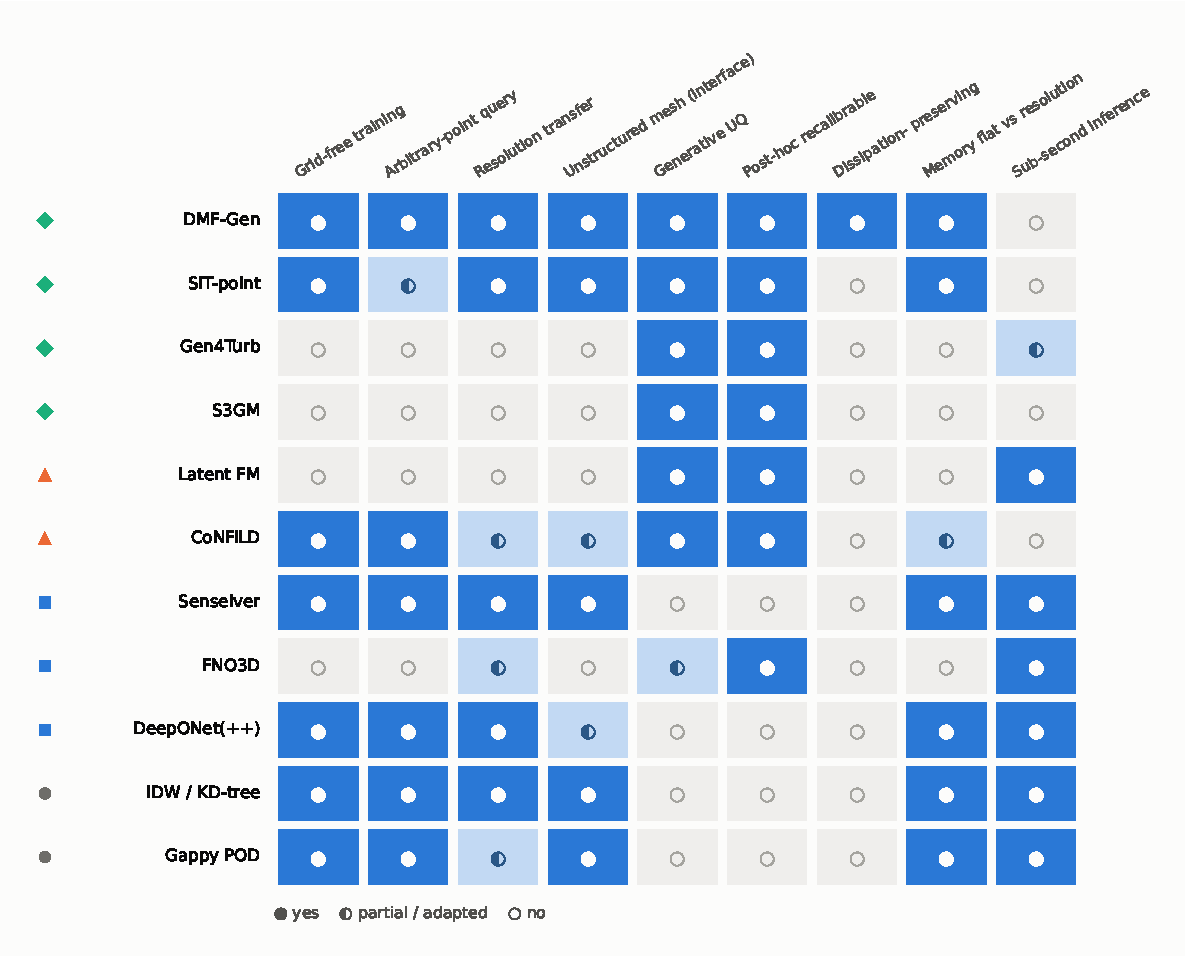
\includegraphics[width=0.92\linewidth]{figures/capability_heatmap.pdf}
\caption{\label{fig:capability}Per-method capability profile across the
deployment axes measured in this paper (filled = yes, half-filled = partial
or adapted, open = no). ``Operator-robust'' records behavior under the
corrupted-operator variants of Sec.~\ref{sec:sensors}, whose full matrix
belongs to the deferred multiphysics regime (Sec.~\ref{sec:discussion});
``dissipation-preserving'' records the windowed dissipation-band ratios
(Sec.~\ref{sec:spectra}); ``memory flat vs
resolution'' and ``sub-second inference'' record the measured scaling study
(Sec.~\ref{sec:cost}). Axes on which a method was not measured are marked
``no'' only when the failure is structural; pending measurements are noted in
the text.}
\end{figure*}

\begin{table}[tbp]
\caption{\label{tab:capability}Capability matrix: which method families can
honestly enter which regimes. RS = requires resampling to a grid (lossy near
the body-fitted boundary of the cylinder mesh); in this suite only the
cylinder exercises that column. $^{\S}$SiT is point-tokenized in the 3D run
but patch-tokenized in both 2D runs, so on the cylinder it consumed the
uniform-grid export rather than the mesh: the family can enter grid-free, this
particular configuration did not.
Every cell in the cylinder column --- the only column that exercises the
resampling distinction --- was checked against the data export the
corresponding run actually opened, not against the family's nominal
capability: Senseiver, MLP-RBF and \dmfgen{} read the 23{,}800-cell mesh,
while Geo-FNO, latent FM, S3GM and SiT read the $400\times200$ grid export.
We keep families rather than one row per method, because the claim the table
makes is about interfaces, and methods inside a family share the interface
even when their accuracy differs by a factor of three.}
\begin{ruledtabular}
\begin{tabular}{lccc}
Family & Cyl. & Kolm. & JHU \\
\hline
Interpolation/POD anchors & \checkmark & \checkmark & \checkmark \\
Point-attention det.\ (Senseiver) & \checkmark & \checkmark & \checkmark \\
Grid det.\ (FNO-class) & RS & \checkmark & \checkmark \\
DeepONet-class & \checkmark & \checkmark & \checkmark \\
Latent-grid generative (LFM) & RS & \checkmark & \checkmark \\
Latent neural-field gen.\ (CoNFiLD) & \checkmark & \checkmark & \checkmark \\
Voxel/video diffusion (Gen4Turb, S3GM) & RS & \checkmark & \checkmark \\
Point-token generative (SiT-point) & RS$^{\S}$ & \checkmark$^{\S}$ & \checkmark \\
Ambient point-cloud FM (\dmfgen{}) & \checkmark & \checkmark & \checkmark \\
\end{tabular}
\end{ruledtabular}
\end{table}

\paragraph{Classical anchors.} Four training-free floors run on every regime:
nearest-neighbor interpolation (KD-tree), inverse-distance weighting over the
$k=8$ nearest sensors, gappy proper orthogonal
decomposition\cite{everson1995karhunen} (POD basis from the training set,
modal coefficients by least squares on the sensor readings, rank 80), and the
training-mean constant. Distance handling is non-periodic by default --- an
earlier periodic implementation understated these floors on non-periodic
cutouts and was corrected in audit --- with periodic variants where the domain
genuinely is periodic. As deterministic point forecasts their CRPS equals
their MAE. These anchors define what any learned method must beat to justify
its training cost.

\paragraph{Deterministic operator learners.} Senseiver\cite{santos2023senseiver}
is an attention-based point-native reconstructor mapping arbitrary sensor sets
to query values through a latent bottleneck; it trains under the identical
sensor randomization as the amortized generative methods. FNO3D places a
spectral (FFT-grid) backbone inside the same conditional-generation framework
as \dmfgen{}, isolating the backbone axis from the formulation axis.
DeepONet\cite{lu2021learning} enters in upstream-faithful form (branch/trunk
with a declared set-encoder adaptation for variable sensor sets); its
near-constant predictions are the pre-registered structural consequence of
global mean pooling in the branch, and a structured-branch redesign
(``DeepONet++'', multiresolution binned pooling) is reported as a labelled
improvement arm. Deterministic models return conditional-mean estimates:
optimal in squared error, systematically smoothed, and structurally unable to
report what the sensors leave undetermined.

\paragraph{Latent generative.} Latent flow matching (LFM) is the
latent-diffusion-family stand-in:\cite{rombach2022high,du2024confild} a
convolutional autoencoder trained on full fields, followed by conditional
rectified flow in its latent space with a point-encoder conditioning branch.
It is the strongest aggregate performer on 3D turbulence and carries the
family's structural signature, a dissipation-range spectral floor inherited
from the autoencoder.\cite{glaws2020deep,rafiq2026spectrally}
CoNFiLD\cite{du2024confild} is the published latent neural-field competitor:
a conditional-neural-field autodecoder compressing each snapshot to a latent
vector, an unconditional diffusion prior over latents, and diffusion posterior
sampling for conditioning; three arms are reported (published prior;
capacity-matched; 384-dimensional), with the latent-capacity ceiling of the
autodecoder measured explicitly as the decoder bound.

\paragraph{Ambient generative.} Gen4Turb\cite{oommen2026turbulent} is voxel
diffusion: an elucidated-diffusion 3D U-Net with mask-channel conditioning,
run at its native $120^3$ on the 3D data and retrained under the benchmark's
observation model (the most generous variant is reported).
S3GM\cite{li2024s3gm} is a pretrained video-diffusion prior with
sampling-time guidance, natively two-dimensional; its 3D entry is a declared
adaptation treating one spatial axis as video time, and its published fixed
guidance weights required tuning-split renormalization to converge at 3D
scale. SiT-point adapts a scalable interpolant transformer\cite{ma2024sit}
with a point tokenizer (not patchification): sensors and queries are tokenized
directly, generation runs in fixed-size token chunks, and the chunk budget is
the visible constraint. That is the 3D configuration; on the two 2D regimes
the same implementation is run patch-tokenized, which is what those rows
report, and on the cylinder it therefore reads the uniform-grid export rather
than the mesh (Table~\ref{tab:capability}) (member-level chunk-incoherent speckle that ensemble
averaging hides --- one reason \benchname{} reports member-level metrics).
\dmfgen{}\cite{wang2026dmfgen} performs conditional rectified flow directly on
field values at scattered points --- ambient function space, no autoencoder,
no voxelization --- with a Gaussian-process source shared across
discretizations, conditioning factored into a global cross-attention summary
plus a local $k$-nearest-sensor retrieval per query, a Monte-Carlo subsampled
training objective (a random ${\sim}2\%$ of points per step), and training
amortized over sensor counts, layouts, noise, and observed-channel subsets. We
evaluate it as published, at the benchmark's parameter budget; it is one row
of the fleet, not the paper's contribution.

\section{Results by regime}\label{sec:results}

\subsection{Laminar vortex shedding: where classical methods should
suffice}\label{sec:cylinder}

The dataset was generated for this benchmark (Sec.~\ref{sec:datasets}) and
verified against the literature before any model saw it: Strouhal numbers
0.140/0.160/0.173/0.187/0.200/0.207 for $Re$ 60--250 track the
Williamson--Norberg correlations, mean drag sits where the 6\% blockage
predicts, and lift amplitude grows monotonically with $Re$. Sensors observe
$(u,v)$ at 1\% of the 23{,}800 mesh cells (238 per field); pressure is never
observed; evaluation is on the held-out Reynolds numbers $\{80, 250\}$.

The classical floors decide this regime before the learned fleet reports.
The training family's POD spectrum is essentially exhausted at rank 20
(99.7\% energy), and \emph{gappy POD with 20 modes reconstructs held-out
Reynolds numbers at 0.056 relative $L_2$ --- including the never-observed
pressure at 0.05} --- because the modal coefficients inferred from sparse
velocities carry the full coupled state. Pure interpolation cannot do this
($p$ column: 1.0 by construction) and trails badly on the velocities as well
(IDW 0.71 aggregate). This is the mirror image of 3D turbulence, where the
same POD basis was useless (0.95, Table~\ref{tab:jhu}) and interpolation was
the strong floor: \emph{which classical method is the one to beat is itself
regime-dependent}, and a learned method only earns its complexity here if it
approaches the POD floor at comparable cost.

It does not, and the gap is resolved rather than marginal: on the same 50
frames and the same seeded draws, rank-20 gappy POD beats the best learned
method by $0.037$ relative $L_2$ (95\% bootstrap CI $[-0.042,-0.032]$,
Wilcoxon $p<10^{-14}$). Table~\ref{tab:cyl} reports the fleet: the closest
learned method, Geo-FNO at 0.093, is still $1.7\times$ the rank-20 POD floor, and the
generative models trail further (latent FM 0.192, \dmfgen{} 0.221, SiT 0.328).
The ordering on the never-observed pressure channel is the sharper statement
--- gappy POD recovers $p$ at 0.043--0.051, better than any learned method
(Geo-FNO 0.088, Senseiver 0.095, \dmfgen{} 0.128) --- because a basis fitted
to the coupled state propagates sparse velocity observations into pressure,
whereas the learned models must infer that coupling from data alone. Read
against Sec.~\ref{sec:identifiability}, where \emph{no} method recovers an
unobserved channel of 3D turbulence, this is the benchmark's cleanest
statement that cross-channel identifiability is a property of the regime and
not of the method class.

Two rows carry caveats rather than results. S3GM diverges here (1.019, worse
than predicting the training mean) under its published predictor--corrector
guidance at this benchmark's parameter budget; we report it as a documented
sampler failure with its diagnostic figures in the artifact rather than
dropping the row, since a benchmark that hides the arms that break is not
measuring robustness. Latent FM is the one over-dispersed model in the suite
(spread--error 1.26, 90\% coverage 0.89 against a 0.90 target), which is what
a calibrated-but-blurry posterior looks like and is consistent with its strong
CRPS at moderate relative $L_2$.

\emph{Which held-out Reynolds number?} The cylinder's held-out set is two
Reynolds numbers, and averaging them hides the more informative question. The
training set is $Re\in\{60,100,150,200\}$, so $Re=80$ is an \emph{interpolation}
in Reynolds number --- bracketed by two training values --- while $Re=250$ lies
past the training maximum and is a genuine \emph{extrapolation}. Splitting the
same 50 canonical frames along that line (Table~\ref{tab:crossre}) gives three
results.

First, the ranking does not change: gappy POD leads at both Reynolds numbers,
Geo-FNO is second at both, Senseiver third at both. The ordering this regime
reports is not an artifact of averaging a hard case with an easy one.

Second, extrapolating costs every working method between $1.26\times$ and
$1.54\times$, and the cost is largest for the \emph{most accurate} rows --- gappy
POD $1.54\times$ (0.044 to 0.068), Geo-FNO $1.50\times$ --- and smallest for the
rows already sitting near the training-mean floor (interpolation $1.11\times$;
diverged S3GM $1.01\times$, which cannot get worse). Methods that exploit the
training family's structure hardest are the ones that lose most when asked to
leave it, which is the honest counterweight to the headline that classical
methods win this regime: gappy POD wins it because the family is low-rank, and
it gives back a larger share of its margin than anything else in the table the
moment the family is left behind.

Third, the never-observed pressure channel is the most Reynolds-sensitive part
of the reconstruction. Six of the seven learned and classical rows that recover
$p$ at all degrade \emph{faster} on $p$ than on their aggregate (gappy POD
$1.73\times$ vs $1.54\times$; Senseiver $1.66\times$ vs $1.26\times$; \dmfgen{}
$1.51\times$ vs $1.30\times$; SiT is the exception at $1.13\times$ vs
$1.31\times$). This is what should be expected and is worth stating because it
is rarely measured: an unobserved channel is reconstructed entirely from
cross-channel structure inferred at the training Reynolds numbers, so it is the
first thing to fail when the flow leaves them. It also explains the
scalar-recalibration failure reported in Sec.~\ref{sec:calibration} --- a single
multiplier fitted across a held-out set spanning an interpolation and an
extrapolation is fitting two different error scales at once.

\begin{table}[tbp]
\caption{\label{tab:crossre}Cylinder cross-Reynolds breakdown of
Table~\ref{tab:cyl}, over the same 50 canonical frames (25 per Reynolds
number). $Re=80$ is an interpolation in $Re$; $Re=250$ is an extrapolation past
the training maximum of 200. Aggregate relative $L_2$, their ratio, and the
never-observed pressure channel. Interpolation rows return the training mean on
$p$ by construction, and their aggregates coincide to four decimals by
coincidence, not by error --- both are dominated by that $p{=}1.0$ column.}
\footnotesize
\begin{ruledtabular}
\begin{tabular}{lccccc}
 & \multicolumn{3}{c}{aggregate} & \multicolumn{2}{c}{$p$ (never observed)} \\
Method & $Re\,80$ & $Re\,250$ & ratio & $Re\,80$ & $Re\,250$ \\
\hline
% GENERATED by src/cross_re_cylinder.py -- do not hand-edit
\dmfgen{} & 0.192 & 0.250 & 1.30 & 0.102 & 0.154 \\
SiT & 0.284 & 0.373 & 1.31 & 0.258 & 0.291 \\
Latent FM & 0.168 & 0.215 & 1.28 & 0.143 & 0.188 \\
S3GM (PC-DPS) & 1.013 & 1.025 & 1.01 & 1.007 & 1.002 \\
Senseiver & 0.129 & 0.162 & 1.26 & 0.071 & 0.118 \\
MLP-RBF & 0.325 & 0.452 & 1.39 & 0.177 & 0.265 \\
Geo-FNO & 0.074 & 0.111 & 1.50 & 0.069 & 0.107 \\
\hline
Gappy POD ($r{=}20$) & 0.044 & 0.068 & 1.54 & 0.037 & 0.064 \\
IDW ($k{=}8$) & 0.667 & 0.742 & 1.11 & 1.000 & 1.000 \\
Nearest neighbour & 0.667 & 0.742 & 1.11 & 1.000 & 1.000 \\
Training mean & 1.000 & 1.000 & 1.00 & 1.000 & 1.000 \\

\end{tabular}
\end{ruledtabular}
\end{table}

\begin{figure}[tbp]
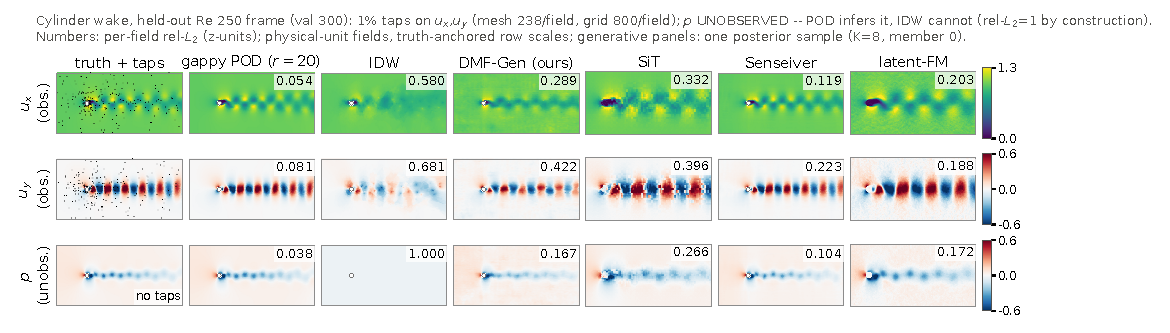
\includegraphics[width=\linewidth]{figures/recon_gallery_cylinder.pdf}
\caption{\label{fig:qual-cyl}Cylinder wake, held-out $\mathrm{Re}=250$ frame,
volume sensing: 1\% of mesh cells on $u_x,u_y$ (black), $p$ never observed.
Single posterior samples, not ensemble means. The $p$ row is the point: gappy
POD infers the unobserved channel through the basis's cross-channel
correlations, while interpolation returns the training mean by construction.}
\end{figure}

\subsection{The same flow, sensed from the surface}\label{sec:surface}

Every result above places sensors throughout the volume. Experiments usually
cannot: a wind-tunnel model carries pressure taps on its skin, and the flow
away from the body is exactly what is unmeasured. We therefore repeat the
cylinder task with sensors confined to the 360 wall-adjacent cells, all three
fields read at the taps and nothing observed off the body, keeping the flow,
the held-out Reynolds numbers, the frames, the seeded-draw machinery and the
training budget identical. Predictions were registered before the runs and are
reported whichever way they fell; two of the three failed.

\emph{The classical floor does not survive the change of geometry.} Gappy POD
with 20 modes wins the volume task outright at 0.056 (Table~\ref{tab:cyl}) and
reaches only 0.689 from the full tap ring, while Senseiver improves from 0.145
to 0.103 and now leads by a factor of $6.7$ over the classical anchor
(Table~\ref{tab:surface}). We had pre-registered the opposite risk --- that
POD might win here too, since the wake is genuinely low-rank --- and it did
not. The reason is that a modal basis needs its coefficients to be
\emph{identifiable} from the measurements, and a boundary ring samples a
one-dimensional manifold on which the leading modes are nearly degenerate;
low-rank structure in the field does not imply well-conditioned inference from
an arbitrary sensor set. Interpolation fails completely, at 2.1 relative $L_2$,
worse than predicting the training mean, because it cannot extrapolate off the
sensor manifold at all.

\emph{The rasterization cost is exact, not approximate.} The 360-cell ring
maps onto only 62 distinct cells of the $400\times200$ export, so every
grid-locked method is blind to tap budgets above 62: Geo-FNO, SiT and latent FM
return bit-identical errors at 64, 128 and 360 taps, to six decimal places,
while the three mesh-native methods keep improving to 360. This is the
capability matrix's ``requires resampling'' column measured rather than
asserted, and it is the clearest evidence in the paper that the interface a
method demands is a scientific property and not an implementation detail.

\emph{What the task does not show.} Grid-locked is not the discriminator:
Geo-FNO places second at 0.119, ahead of every point-native generative model.
The surface geometry separates deterministic from generative methods, the
reverse of what we expected from the argument that an under-determined
far-wake posterior should reward a calibrated distribution. \dmfgen{} is
fourth at 0.245 and does not lead on CRPS either. We record the failed
prediction rather than reframing it.

% Rows generated by src/figs_pof/make_surface_table.py from
% Save_TrainedModel/cylinder2d_surface/**/Evaluation/cyl_surface_*.json
\begin{table}[tbp]
\caption{\label{tab:surface}Cylinder \emph{surface-to-field}: reconstruct the
full wake from taps on the body alone, held-out $\mathrm{Re}\in\{80,250\}$,
50 Re-stratified frames. Columns are taps per field on the 360-cell wall ring;
all three fields are read at the taps and nothing is observed off the body.
$\dagger$ = identical to the 64-tap entry by construction: the ring rasterizes
onto 62 grid cells, so grid-locked methods cannot represent a larger budget.
Compare with Table~\ref{tab:cyl}, the same flow sensed in the volume, where
the ranking is inverted.}
\footnotesize
\begin{ruledtabular}
\begin{tabular}{lccccc}
 & \multicolumn{4}{c}{Rel.\ $L_2$ at $n$ taps/field} & \\
\cline{2-5}
Method & 32 & 64 & 128 & 360 & CRPS \\
\hline
% GENERATED by src/figs_pof/make_surface_table.py -- do not hand-edit
Senseiver & 0.109 & 0.105 & 0.104 & \textbf{0.103} & 0.058 \\
Geo-FNO & 0.161 & 0.119 & 0.119 & 0.119 & 0.073 \\
\dmfgen{} & 0.271 & 0.252 & 0.247 & 0.245 & 0.111 \\
MLP-RBF & 0.337 & 0.307 & 0.269 & 0.246 & 0.138 \\
SiT & 0.494 & 0.476 & 0.476 & 0.476 & 0.180 \\
Latent FM & 0.631 & 0.569 & 0.569 & 0.569 & 0.220 \\
S3GM & 0.897 & 0.891 & 0.891$^\dagger$ & 0.891$^\dagger$ & 0.468 \\
\hline
Gappy POD ($r{=}20$) & 1.223 & 0.919 & 0.781 & 0.689 & 0.306 \\
IDW ($k{=}8$) & 2.077 & 2.117 & 2.132 & 2.141 & 1.937 \\
Nearest neighbour & 2.159 & 2.153 & 2.148 & 2.144 & 1.940 \\

\end{tabular}
\end{ruledtabular}
\end{table}

\begin{figure}[tbp]
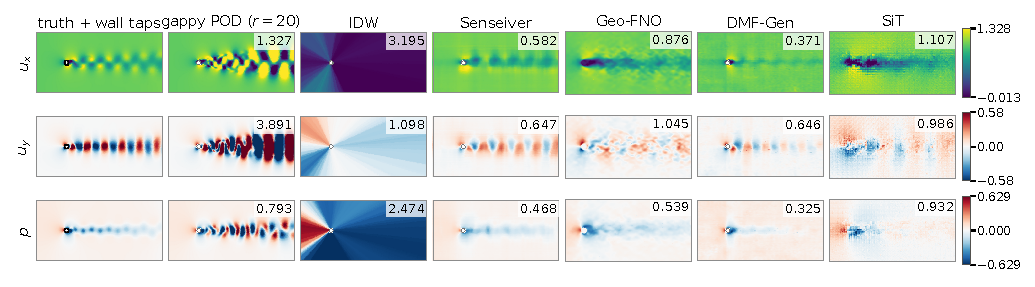
\includegraphics[width=\linewidth]{figures/recon_gallery_cylinder_surface.pdf}
\caption{\label{fig:qual-surface}Surface-only sensing on the held-out
$\mathrm{Re}=250$ frame: taps (black) sit on the body, everything else is
inferred. Read against Fig.~\ref{fig:qual-cyl}, the identical frame sensed in
the volume.}
\end{figure}

% Rows generated from the canonical JSONs by src/figs_pof/make_2d_tables.py.
% Sources: Save_TrainedModel/cylinder2d/*/*/Evaluation/cyl_fleet_*.json (n=50,
%   K=8 generative / K=1 deterministic) and baseline_classical/
%   classical_baselines_main_1pct_pod{20,80}_2d.json (all 600 held-out frames).
\begin{table}[tbp]
\caption{\label{tab:cyl}Cylinder wake, cross-$\mathrm{Re}$ evaluation on the
held-out $\mathrm{Re}\in\{80,250\}$ ($u,v$ observed at 1\% = 238 sensors per
field on the 23{,}800-cell mesh; \emph{$p$ is never observed}; learned rows:
50 Re-stratified held-out frames, $K{=}8$; classical floors: all 600).
Deterministic rows carry $K{=}1$ and null dispersion. Interpolation returns
the training mean on the unobserved channel, hence $p{=}1.000$ by
construction.}
\footnotesize
\begin{ruledtabular}
\begin{tabular}{lccccccc}
 & \multicolumn{4}{c}{Rel.\ $L_2$} & & & \\
\cline{2-5}
Method & agg. & $u_x$ & $u_y$ & $p$ & CRPS & Cov.$_{90}$ & s/field \\
\hline
% GENERATED by src/figs_pof/make_2d_tables.py -- do not hand-edit
\dmfgen{} (NFE 4) & 0.221 & 0.182 & 0.353 & 0.128 & 0.098 & 0.51 & 0.08 \\
SiT (50 steps) & 0.328 & 0.302 & 0.409 & 0.274 & 0.106 & 0.55 & 0.19 \\
Latent FM (NFE 4) & 0.192 & 0.170 & 0.239 & 0.166 & 0.076 & 0.89 & 0.03 \\
S3GM (PC-DPS) & 1.019 & 1.035 & 1.017 & 1.005 & 0.521 & 0.58 & 29.24 \\
Senseiver & 0.145 & 0.101 & 0.240 & 0.095 & 0.080 & --- & 0.01 \\
MLP-RBF & 0.388 & 0.265 & 0.679 & 0.221 & 0.213 & --- & 0.01 \\
Geo-FNO & 0.093 & 0.087 & 0.103 & 0.088 & 0.053 & --- & 0.01 \\
\hline
Gappy POD ($r{=}20$) & \textbf{0.056} & 0.043 & 0.075 & 0.051 & 0.029 & --- & --- \\
Gappy POD ($r{=}80$) & 0.067 & 0.055 & 0.103 & \textbf{0.043} & 0.028 & --- & --- \\
IDW ($k{=}8$) & 0.707 & 0.504 & 0.616 & 1.000 & 0.440 & --- & --- \\
Nearest neighbour & 0.707 & 0.508 & 0.613 & 1.000 & 0.421 & --- & --- \\
Training mean & 1.000 & 1.000 & 1.000 & 1.000 & 0.664 & --- & --- \\

\end{tabular}
\end{ruledtabular}
\end{table}

\subsection{Two-dimensional Kolmogorov turbulence}\label{sec:kolmogorov}

Sensors observe vorticity at 1\% of the $256^2$ points (655 sensors);
learned models are scored on 50 evenly spaced frames of the eight held-out
trajectories ($K{=}8$, identical canonical seeded draws across methods;
classical floors on all 640). Table~\ref{tab:kolm} reports the full fleet
alongside the floors, and Fig.~\ref{fig:sensors} (left) the sensor-count
sweep. Three regime findings stand out.

First, \emph{the 3D ranking does not transfer}. Geo-FNO wins relative $L_2$
outright at 0.385 --- 21\% better than the best generative model --- while
latent FM, the 3D aggregate winner, trails even the interpolation floor here
(0.599 against 0.531) at the matched ${\sim}50$k-step budget. The remaining
generative models land between them (\dmfgen{} 0.487, SiT 0.494, S3GM 0.498);
of these only \dmfgen{} is ambient point-based here, since SiT and S3GM are
run patch- and voxel-tokenized on this grid. The two deterministic point
models split: MLP-RBF at 0.639 and Senseiver at 0.913, the latter barely
inside the training-mean floor.

Second, \emph{the accuracy and the probabilistic ranking disagree across
method families, not within them}. The same Geo-FNO row that wins relative
$L_2$ is beaten on CRPS by every generative model (0.267 against S3GM 0.231,
SiT 0.234, \dmfgen{} 0.235). This is the distortion--perception tradeoff of
Sec.~\ref{sec:dp} appearing as a family-level split rather than a curve: a
conditional-mean estimator minimizes squared error and is then penalized by a
proper score that rewards a calibrated distribution. Reporting either metric
alone would name a different winner, which is why the benchmark requires both.

The winning row initially received more training than the rest, and we
retrained it to check. The Kolmogorov budget was set in \emph{epochs} (2500) at
batch size 128, giving the ${\sim}50$k optimizer steps every other row
receives: Senseiver 50.0k, MLP-RBF 50.0k, latent FM 50.0k, \dmfgen{} 51.2k,
S3GM 51.2k, SiT 52.0k. Geo-FNO inherited the same epoch count at batch size 32,
which is 80 rather than 20 steps per epoch and therefore 200k steps, four times
the fleet budget. Matching budgets by epoch count rather than by step count is
an easy error to make when batch sizes differ across a fleet, and it is why
this benchmark reports as-run steps per row.

Retrained at exactly 50k steps (625 epochs, configuration otherwise
untouched), \emph{Geo-FNO still wins}: 0.417 relative $L_2$ against
\dmfgen{}'s 0.487, SiT's 0.494 and S3GM's 0.498. The margin narrows from 21\%
to 14.5\% and the ordering is unchanged, with the paired difference resolved
against all three ($-0.060$, CI $[-0.068,-0.053]$ versus \dmfgen{};
$p<10^{-14}$ in every case) and roughly fifteen times the training-seed spread.
The four-fold budget was worth 0.032 relative $L_2$ to this architecture --- a
real effect, and smaller than the gap it was suspected of manufacturing. We
report the matched number as the row and the over-trained one as an ablation,
because the leaderboard should answer what a method achieves at the benchmark's
budget.

Third, the floors carry regime information of their own: gappy POD's rank-80
training basis captures only 70.5\% of the training-set energy ---
two-dimensional turbulence is not low-rank in the POD sense, unlike the
cylinder --- and plain inverse-distance weighting beats it by 20\% relative
$L_2$.

All comparisons here are paired: every method is scored on the same 50 frames
under the same seeded draws, so the per-snapshot difference is the unit of
analysis. We report the mean paired difference with a 95\% percentile
bootstrap interval (20{,}000 resamples) and call a gap resolved only when the
interval excludes zero \emph{and} a Wilcoxon signed-rank test agrees at
$p<0.05$. Geo-FNO's lead is resolved against the whole fleet (against
\dmfgen{}, $-0.103$, CI $[-0.112,-0.094]$, $p<10^{-14}$), whereas the three
generative models behind it are not separable from each other: \dmfgen{} versus
SiT gives $-0.006$ with $p=0.16$, and SiT versus S3GM $-0.004$ with $p=0.32$.
Only the \dmfgen{}--S3GM pair separates ($-0.010$, $p=0.008$), which is the
expected intransitivity when three methods sit inside a 0.011 band --- we
therefore report them as a tie group rather than ranking them.

Retraining answers the same question from the other side. Each 2D method was
retrained from scratch under two further seeds (7 and 1337, configurations
otherwise identical) and re-evaluated under the frozen protocol. Training-seed
spread is small: pooled standard deviation 0.0041 relative $L_2$ across the
full Kolmogorov fleet and 0.0081 on the cylinder. The most seed-sensitive row
is S3GM in both regimes (0.0082 and 0.0163), which is consistent with the
sampler fragility documented elsewhere; the least is SiT on Kolmogorov
(0.0006). Every adjacent gap in the cylinder ranking exceeds the pooled spread
by at least a factor of $3.7$ --- the tightest being latent FM against
\dmfgen{} at 0.030 --- so that ordering is seed-robust end to end, though by a
smaller margin than the accuracy gaps alone suggest. On Kolmogorov the same test isolates the
same tie group the paired intervals found: Geo-FNO's lead over \dmfgen{} is
0.103, twenty-five times the seed spread, while \dmfgen{}--SiT (0.006) and
SiT--S3GM (0.004) are one to one-and-a-half seed standard deviations apart and
cannot be called ordered. Two
independent notions of uncertainty --- resampling the evaluation frames and
resampling the training run --- agree on which comparisons this benchmark
resolves, which is the reassurance a leaderboard needs before anyone builds on
its ordering.
\todo{operator variants (Sec.~\ref{sec:sensors}).}

% Sources: Save_TrainedModel/kolmogorov2d/baseline_classical/
%   classical_baselines_main_1pct_{nonperiodic,periodic}_2d.json;
%   kolm_fleet_{dmfgen,sit,latentfm}_*.json (job 17938333, 50 frames, K=8)
\begin{table}[tbp]
\caption{\label{tab:kolm}Kolmogorov $256^2$, trajectory-holdout evaluation
(vorticity observed at 1\% = 655 sensors, identical canonical seeded draws;
learned rows: 50 evenly spaced held-out frames, $K{=}8$; classical floors:
all 640). Deterministic rows carry $K{=}1$ and null dispersion, so their
coverage cell is empty and their CRPS equals the MAE exactly. Inference cost
per field on one H100. Rows are generated from the canonical JSONs by
\texttt{src/figs\_pof/make\_2d\_tables.py}.}
\footnotesize
\begin{ruledtabular}
\begin{tabular}{lccccc}
Method & Rel.\ $L_2$ & CRPS & Cov.$_{90}$ & s/field & GB \\
\hline
% GENERATED by src/figs_pof/make_2d_tables.py -- do not hand-edit
\dmfgen{} (NFE 4) & 0.487 & 0.578 & 0.235 & 0.59 & 0.28 & 0.76 \\
SiT (50 steps) & 0.494 & 0.590 & 0.234 & 0.64 & 0.18 & 0.24 \\
Latent FM (NFE 4) & 0.599 & 0.731 & 0.310 & 0.64 & 0.03 & 0.19 \\
S3GM (PC-DPS) & 0.498 & 0.700 & \textbf{0.231} & 0.80 & 22.05 & 17.42 \\
Senseiver & 0.913 & 0.913 & 0.697 & --- & 0.01 & 0.71 \\
MLP-RBF & 0.639 & 0.639 & 0.469 & --- & 0.01 & 0.79 \\
Geo-FNO & \textbf{0.417} & \textbf{0.417} & 0.287 & --- & 0.01 & 0.34 \\
\hline
IDW ($k{=}8$) (per.) & 0.531 & 0.531 & 0.375 & --- & --- & --- \\
IDW ($k{=}8$) (non-per.) & 0.546 & 0.546 & 0.385 & --- & --- & --- \\
Nearest neighbour (per.) & 0.582 & 0.582 & 0.371 & --- & --- & --- \\
Nearest neighbour (non-per.) & 0.588 & 0.588 & 0.375 & --- & --- & --- \\
Gappy POD ($r{=}80$) & 0.680 & 0.680 & 0.510 & --- & --- & --- \\
Training mean & 1.000 & 1.000 & 0.753 & --- & --- & --- \\

\end{tabular}
\end{ruledtabular}
\end{table}

\begin{figure}[tbp]
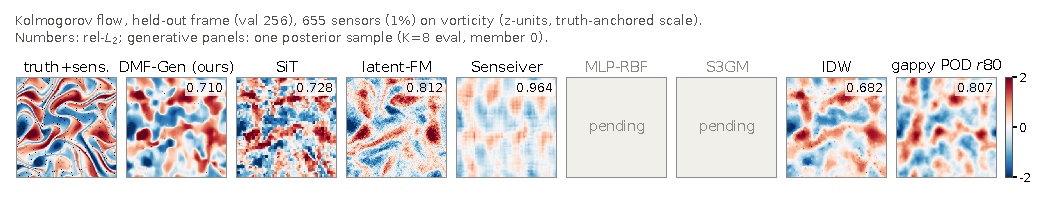
\includegraphics[width=\linewidth]{figures/recon_gallery_kolmogorov.pdf}
\caption{\label{fig:qual-kolm}Kolmogorov $256^2$, canonical held-out frame,
vorticity at 1\% sensing. Single posterior samples. Gappy POD is visibly
over-smoothed --- two-dimensional turbulence is not low-rank --- while the
generative samples carry small-scale texture that the deterministic rows lack
even where their pointwise error is lower.}
\end{figure}

\subsection{Three-dimensional isotropic turbulence: the full
fleet}\label{sec:jhu}

The 3D turbulence benchmark is the controlled comparison: a periodic-topology
regular grid is native terrain for voxel, patchified, and latent-grid methods,
so every family competes at full strength. Sensors observe $U_x$ and $U_z$ at
1\% of $1.95\times10^{6}$ points per channel; $U_y$ and $p$ are never
observed. Table~\ref{tab:jhu} reports per-channel accuracy and probabilistic
scores for the full fleet on all 50 held-out snapshots of the spatially
disjoint cutout under canonical seeded draws; Table~\ref{tab:jhucost} reports
the matched cost accounting.

% Source: FLEET_SUMMARY_TABLE_2026-08-30.md (canonical n=50 JSONs)
\begin{table*}[tbp]
\caption{\label{tab:jhu}3D isotropic turbulence, spatially disjoint
evaluation region ($1.95$M points; $U_x,U_z$ observed at 1\% per channel,
$U_y^*,p^*$ unobserved; canonical seeded sensor draws, all $n{=}50$ held-out
snapshots, $K{=}8$ ensembles at each method's listed sampler setting).
Per-channel relative $L_2$ of the ensemble mean is primary; agg$^\dagger$
averages all four channels and is flagged, not headlined. Unobserved-channel
error $\ge 1.0$ is worse than predicting the training mean; values near 1.0
across the fleet reflect a shared identifiability limit of point-conditioned
methods (Sec.~\ref{sec:identifiability}). Spread--error and coverage ideals
are 1.0 and 0.90; for deterministic methods CRPS reduces to MAE and
dispersion is undefined. Step budgets are as-run, not equalized
(Table~\ref{tab:jhucost}). Labelled improvement arms (Senseiver capacity,
DeepONet++, CoNFiLD repairs, S3GM normalized guidance) are reported in the
artifact. $^{\ddagger}$ = guidance deviates from the published setting, which
is why the upstream-faithful S3GM row is reported separately above it rather
than replaced by the working one; the normalized-guidance coefficients were
fitted on the tuning split only, and its tune/test difference is below 0.001
relative $L_2$. A CoNFiLD strict-2048 arm was
run and is deliberately \emph{not} in this table. Its 50 per-snapshot files
aggregate to rel-$L_2$ 0.941 / CRPS 0.500 ($U_x$ 0.525, $U_z$ 0.559) rather
than the 0.90 recorded for it earlier, and they carry no protocol stamp --- no
sensor count, conditioned channels, seed or $K$ --- so there is no way to
confirm from the artifact that it saw the canonical sensor draw. We report it
here in the text rather than as a row, because admitting a number to a
comparison table on the strength of its filename is exactly the failure this
benchmark exists to argue against.}
\footnotesize
\begin{ruledtabular}
\begin{tabular}{lcccccccc}
Method & $U_x$ & $U_y^*$ & $U_z$ & $p^*$ & agg$^\dagger$ & CRPS & Spr/Err & Cov.$_{90}$ \\
\hline
\dmfgen{} (NFE 4) & 0.176 & 1.048 & 0.182 & 0.964 & 0.593 & 0.291 & 0.63 & 0.54 \\
Latent flow matching & 0.248 & \textbf{0.727} & 0.257 & \textbf{0.646} & \textbf{0.469} & \textbf{0.244} & 0.68 & 0.56 \\
SiT-point ($N{=}32$) & \textbf{0.143} & 0.968 & \textbf{0.132} & 0.937 & 0.545 & 0.338 & 0.75 & 0.58 \\
FNO3D (same framework, NFE 4) & 0.188 & 0.904 & 0.191 & 1.061 & 0.586 & 0.269 & \textbf{0.94} & \textbf{0.63} \\
CoNFiLD (published prior, DPS 1000) & 0.409 & 0.751 & 0.374 & 1.007 & 0.635 & 0.371 & 0.82 & 0.57 \\
CoNFiLD (capacity-matched) & 0.488 & 1.089 & 0.420 & 1.487 & 0.871 & 0.562 & 0.62 & 0.45 \\
CoNFiLD (384-d) & 0.524 & 0.604 & 0.451 & 1.401 & 0.745 & 0.480 & 0.69 & 0.50 \\
Gen4Turb (anneal, 32-step) & 0.224 & 0.996 & 0.455 & 1.005 & 0.670 & 0.407 & 0.37 & 0.33 \\
S3GM (upstream guidance, $N{=}200$) & \multicolumn{8}{c}{diverges at 3D scale (rel-$L_2$ $8.9{\times}10^{5}$); see text} \\
S3GM (retuned guidance)$^{\ddagger}$ & 0.362 & 0.992 & 0.350 & 1.024 & 0.682 & 0.368 & 0.48 & 0.42 \\
S3GM (normalized guidance)$^{\ddagger}$ & 0.260 & 0.980 & 0.254 & 1.018 & 0.628 & 0.343 & 0.52 & 0.46 \\
\hline
Senseiver (deterministic) & 0.361 & 1.077 & 0.380 & 0.978 & 0.699 & 0.479 & --- & --- \\
DeepONet (deterministic) & 0.593 & 0.972 & 0.652 & 0.985 & 0.800 & 0.570 & --- & --- \\
\hline
Nearest neighbor (KD-tree) & 0.209 & 1.000 & 0.219 & 1.000 & 0.607 & 0.406 & --- & --- \\
IDW ($k{=}8$, non-periodic) & 0.174 & 1.000 & 0.181 & 1.000 & 0.589 & 0.396 & --- & --- \\
Gappy POD ($r{=}80$) & 0.523 & 1.306 & 0.540 & 1.443 & 0.953 & 0.673 & --- & --- \\
Training mean & 1.000 & 1.000 & 1.000 & 1.000 & 1.000 & 0.786 & --- & --- \\
\end{tabular}
\end{ruledtabular}
\end{table*}

\begin{figure}[tbp]
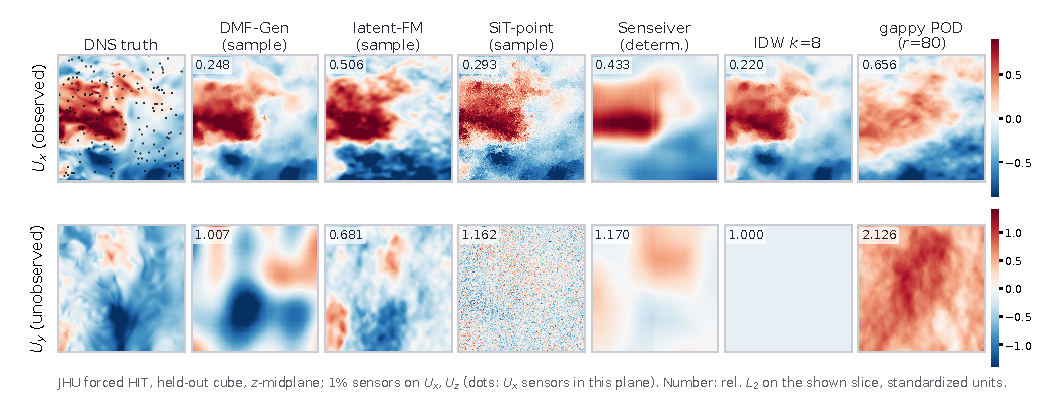
\includegraphics[width=\linewidth]{figures/recon_gallery_jhu.pdf}
\caption{\label{fig:qual-jhu}3D isotropic turbulence, held-out cutout, $z$
mid-slice: $U_x,U_z$ observed at 1\%, $U_y$ and $p$ never observed. Single
posterior samples. The unobserved rows are the identifiability wall of
Sec.~\ref{sec:identifiability}: every method produces plausible texture with
no pointwise agreement.}
\end{figure}

% Source: FLEET_SUMMARY_TABLE_2026-08-30.md
\begin{table*}[tbp]
\caption{\label{tab:jhucost}Cost accounting for the 3D-turbulence fleet
(H100-SXM 80\,GB). Steps are as-run, not equalized: every external baseline
received at least \dmfgen{}'s 48k optimizer steps except SiT-point
(wall-clock-matched, 38.5k); CoNFiLD stages train on a wall-clock budget.
``(d)'' = derived from evaluation-job wall time rather than a dedicated
benchmark, and therefore an \emph{upper bound}: it includes data loading,
host--device transfer and metric computation, which the dedicated numbers
exclude. The two kinds are not interchangeable and we mark rather than mix
them; the marked rows are the slow samplers, where the sampling term dominates
the overhead and the comparison it supports (orders of magnitude between
families) is unaffected. Unifying them would mean re-benchmarking every row on
one device, and the H100s these numbers were taken on are no longer the
project's hardware, so the honest options are to keep the marked mixture or to
re-measure the whole table on the current GPUs; we keep the mixture rather
than silently restate the hardware.}
\footnotesize
\begin{ruledtabular}
\begin{tabular}{lcccccc}
Method & Params & Opt.\ steps & Train s/step & Train GPU-h & Train peak GB & Infer s/field \\
\hline
\dmfgen{} (NFE 4) & 6.51M & 48k & 0.574 & 7.7 & 53.6 & ${\sim}$17 (d) \\
Latent flow matching & 6.68M & 209k$+$95k & 0.238 & 13.9 & 3.6 & 0.019 \\
SiT-point ($N{=}32$) & 6.57M & 38.5k & 1.81 & 19.4 & 26.8 & ${\sim}$150 (d) \\
FNO3D (NFE 4) & 6.73M & 79.9k & 0.766 & 17.0 & 48.6 & 0.097 \\
CoNFiLD (pub.\ prior) & 118.9M$^{w}$ & wall & 35.5/ep & ${\sim}$19 & 4.7 & ${\sim}$130 (d) \\
Gen4Turb (anneal) & 6.16M & 105k & 0.598 & 17.4 & 47.4 & 1.65 \\
S3GM (JHU-tuned) & 6.35M & 105k & 0.635 & 18.5 & 26.3 & ${\sim}$46 \\
Senseiver & 6.42M & 79.2k & 0.776 & 17.0 & 22.4 & $<$1 \\
DeepONet & 6.51M & 82.0k & 0.29 & 6.7 & 15.7 & 0.23 \\
IDW $k{=}8$ (CPU) & --- & --- & --- & --- & 10 (RSS) & 0.68 \\
Gappy POD $r{=}80$ (CPU) & --- & 45\,s fit & --- & --- & 10 (RSS) & 0.14 \\
\end{tabular}
\end{ruledtabular}
\end{table*}

The honest headline is that no method leads every column. SiT-point posts the
best observed-channel errors (0.143/0.132) at roughly 150\,s per field ---
239 sequential 8{,}192-token chunks at 32 steps --- and its single samples
carry chunk-incoherent speckle that the ensemble mean averages away. Latent
flow matching leads the aggregate, the unobserved channels, and CRPS: its
convolutional decoder emits globally structured fields even where no sensor
constrains them, at the dissipation-range price quantified in
Sec.~\ref{sec:spectra}. Non-periodic inverse-distance weighting --- a
training-free interpolant --- edges the best learned observed-channel error
(0.174 vs.\ 0.176 on $U_x$ for \dmfgen{}), so no learned method beats
interpolation on observed channels at 1\% density; the learned and generative
payoffs concentrate where the problem is ill-posed --- unobserved channels,
sparser sensing --- and in sampling cost (\dmfgen{} reaches its accuracy in
4 network evaluations against 32--1000 for the guided-diffusion and
transformer baselines).
DeepONet's near-constant predictions are the structural consequence of global
mean pooling in its branch; the labelled DeepONet++ arm (structured pooling)
improves $U_x$ from 0.593 to 0.512 and remains behind the point-attention
family.

S3GM needs its three rows read together, because reporting only the first
would misrepresent the method. At the published guidance coefficients
($\alpha_{\rm case}{=}0.5$, $\beta{=}0.4$) the sampler diverges at this scale
by five orders of magnitude, and we verified that each coefficient diverges
independently --- this is a property of the guidance at $1.95$M points, not a
porting defect, and the archived divergence figures are documentation of the
failure rather than a model result. Reducing both coefficients by two orders
of magnitude makes the sampler stable and it then scores 0.682 aggregate;
replacing the guidance with a normalized form whose coefficients are fitted on
the tuning split reaches 0.628 with observed-channel errors of 0.260 and
0.254. Both are labelled deviations from the published method, so neither can
be quoted as ``S3GM'' without qualification, and neither closes the
unobserved-channel gap (0.98--1.02) that no method in the fleet closes. The
benchmark's rule --- evaluate as published, then report labelled repairs
separately --- is what makes the distinction visible instead of a footnote.

The top of this table is partly a tie. Applying the paired analysis of
Sec.~\ref{sec:kolmogorov} to the canonical $n{=}50$ JSONs, latent FM's lead is
resolved against both of the rows immediately behind it (against FNO3D
$-0.118$, CI $[-0.147,-0.088]$; against \dmfgen{} $-0.124$, CI
$[-0.147,-0.102]$; both $p<10^{-9}$), while FNO3D and \dmfgen{} are not
separable from each other ($-0.007$, CI $[-0.027,+0.015]$, $p=0.33$) despite
being reported as different rows. A ranking that reads the third and fourth
entries as ordered would be over-reading the benchmark's resolution at this
$n$.

Two limits on that statement are worth being explicit about, because both bound
what this table can support. First, only the three rows above could be compared
frame by frame: the SiT-point, Senseiver, Gen4Turb and DeepONet rows have no
canonical per-snapshot payloads in the artifact set (SiT and Gen4Turb have
none; Senseiver's predate the current schema), and a paired test cannot be
reconstructed from an aggregate. Their positions in Table~\ref{tab:jhu} are
therefore point estimates without a paired interval, and we do not claim
any of them is separated from a neighbour. Second, the seed error bar reported
in this paper covers the two 2D regimes only
(Sec.~\ref{sec:kolmogorov}); the 3D rows are single training runs, so the
resolution argument above rests on evaluation-frame resampling alone rather
than on both notions of uncertainty. Where a 3D comparison is called resolved
it is resolved in that weaker sense, and we flag it rather than let the 2D
seed study stand in for a measurement we did not make at 3D scale.

\section{Cross-cutting analyses}\label{sec:analysis}

\subsection{The distortion--perception tradeoff, operationally}\label{sec:dp}

Relative $L_2$ of the ensemble mean is minimized by the posterior mean --- by
construction it rewards collapse toward a smooth conditional average --- while
proper scores and physics metrics reward calibrated diversity and sharp
members. The benchmark measures the tension directly through the sampler's
operating point: for the rectified-flow methods, two integration steps give
the best mean-field error and the sharpest single samples, four steps are the
CRPS optimum, and dispersion rises monotonically with further steps at flat
CRPS (spread--error 0.65 at NFE 2 to 0.92 at NFE 16 for the
$\lambda_{\mathrm{sp}}{=}0$ \dmfgen{} variant). A spectral training penalty
moves along the same frontier: it buys single-sample sharpness and
inertial-band fidelity at a measured cost in dispersion. The practical rule
the benchmark enforces: never rank generative reconstruction methods on
mean-field error alone, and attach the sampler operating point to every
probabilistic number.

\subsection{Unobserved channels: a fleet-wide identifiability
limit}\label{sec:identifiability}

\begin{figure*}[t]
\centering
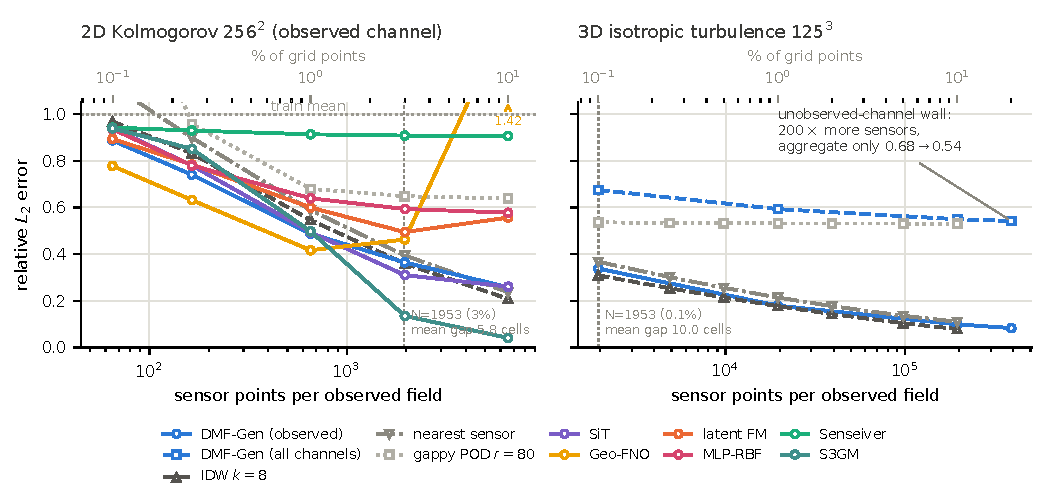
\includegraphics[width=\textwidth]{figures/perf_vs_sensors}
\caption{\label{fig:sensors}Reconstruction error versus the \emph{number} of
sensor points, in 2D (left, Kolmogorov $256^2$, the full learned fleet) and 3D
(right, JHU $125^3$ cross-cube; solid = observed-channel rel-$L_2$, dashed =
aggregate over all four channels). Colored = learned; gray = classical floors.
The two panels sit on opposite sides of the density story: the same sensor
count that leaves a 5.8-cell mean gap in 2D leaves a 10-cell gap in 3D, and
while every 3D observed-channel error falls steadily with sensor count ---
\dmfgen{} tracking the interpolation slope from 0.33 to 0.09 over $200\times$
--- the 3D \emph{aggregate} saturates near 0.54 because the unobserved
channels do not identify (Sec.~\ref{sec:identifiability}). Gappy POD is flat
at every 3D density: isotropic turbulence has no low-rank structure for added
sensors to project onto. In 2D the fleet fans out rather than sharing a slope:
four rows fall monotonically, Geo-FNO and latent FM \emph{degrade} past
$\sim$2000 sensors, and Senseiver is nearly flat throughout. Learned rows:
canonical protocol, 50 held-out frames, $K$ as in Table~\ref{tab:kolm};
classical curves: same seeded sensor draws. S3GM's sweep is still running.}
\end{figure*}

Before the unobserved-channel story, the 2D panel settles a question the
single-density tables cannot: \emph{over what range of sensor budgets does
learning pay for itself?} Sweeping the Kolmogorov fleet over
$\{65,164,655,1965,6554\}$ sensors --- $0.1\%$ to $10\%$ of the grid, canonical
draws at every density --- bounds that range on both sides. At the sparse end
learning wins clearly: at 65 sensors Geo-FNO reaches 0.776 and \dmfgen{} 0.887
while IDW manages only 0.968 and gappy POD (1.82) and nearest-sensor (1.12) are
both worse than predicting the training mean. At the dense end the ordering
inverts: at 6554 sensors plain inverse-distance interpolation reaches 0.208 and
beats \emph{every} learned row in the fleet, the best of which are \dmfgen{} at
0.258 and SiT at 0.261. The crossover falls between 1965 and 6554 sensors, i.e.
between roughly $3\%$ and $10\%$ of the grid --- so on this flow the entire case
for a learned reconstructor lives below a few percent sensing, which is
precisely the regime the benchmark targets and precisely the regime that
uniform-downsampling protocols leave (Sec.~\ref{sec:leakage}).

The fleet also does not share a slope, and the exceptions are diagnostic rather
than noisy. Four rows fall monotonically over the full $100\times$ range
(\dmfgen{} $0.887\!\to\!0.258$, SiT $0.940\!\to\!0.261$, MLP-RBF
$0.936\!\to\!0.578$, Senseiver $0.942\!\to\!0.907$). Two do not: Geo-FNO
improves to 0.332 at 1965 sensors and then \emph{degrades to 0.696} at 6554,
and latent FM turns the same corner more gently ($0.495\!\to\!0.557$). Both are
the rows whose conditioning path resamples the sensors onto a fixed
representation --- a grid for Geo-FNO, a latent code for latent FM --- so
adding sensors past the point where that representation saturates adds
conditioning mismatch rather than information. This is a failure mode a
single-density leaderboard cannot see at all: at the canonical $1\%$ row
Geo-FNO is the best learned method on this regime (Table~\ref{tab:kolm}), and
nothing in that number warns a practitioner that ten times the instrumentation
would make it twice as bad. Senseiver's near-flatness is the same lesson from
the other direction --- it extracts essentially all it will ever extract from
65 sensors --- and is why we report the density sweep as a first-class result
rather than an appendix curve.

On 3D turbulence, no method in the fleet reconstructs the unobserved $U_y$
below 0.60 relative $L_2$, and most sit near or above 1.0 --- worse than
predicting the training mean (Table~\ref{tab:jhu}). The two partial
exceptions (latent FM at 0.727, CoNFiLD-384d at 0.604) are the two methods
whose decoders impose the strongest global field structure, and both pay for
it elsewhere (dissipation-range truncation; observed-channel accuracy). This
is not a per-method defect: at 1\% point sensing on two velocity components,
the instantaneous realization of a third component of 3D turbulence is close
to unidentifiable, and only its statistics are recoverable. The observation
disciplines how such results should be reported --- per channel, with
unobserved channels flagged --- and motivates the cylinder's
observe-$u$-only variant, where the shedding phase \emph{does} determine the
unobserved channels and the same test separates methods rather than hitting
a physics ceiling. The cylinder's own never-observed pressure channel already
makes the contrast quantitative: where 3D turbulence compresses every method
into the 0.90--1.00 band, the same measurement on the cylinder spreads them
over more than an order of magnitude --- gappy POD 0.043, Geo-FNO 0.088,
Senseiver 0.095, \dmfgen{} 0.128, SiT 0.274, and interpolation at 1.000 by
construction (Table~\ref{tab:cyl}). Identifiability is therefore a property of
the flow and the sensing geometry, not a fixed limitation of a method class,
and a benchmark that reports only 3D would license the wrong conclusion.

The observe-$u$-only arm makes the point sharper still. Retraining on
$u_x$ sensors alone --- so that $u_y$ joins $p$ as an unobserved channel, and
the total sensor budget halves from 476 to 238 --- leaves Senseiver's $u_y$
error unchanged at 0.231, against 0.240 when $u_y$ was measured directly at
1\%. Removing an entire observed channel costs it nothing, because at this
Reynolds number the shedding phase inferred from $u_x$ determines the rest of
the field; its aggregate moves only from 0.145 to 0.148. \dmfgen{} is not
indifferent in the same way: its $u_y$ error rises from 0.353 to 0.438 and its
aggregate from 0.221 to 0.250. The contrast with Table~\ref{tab:jhu}, where no
method recovers an unobserved channel of 3D turbulence at any budget, is the
cleanest statement the benchmark makes about identifiability: whether a
channel is recoverable is set by the flow, and \emph{how efficiently a method
exploits that recoverability} is what separates architectures. Reporting only
the aggregate would hide both halves.

\subsection{Calibration: characterized, then repaired}\label{sec:calibration}

Almost every scored ensemble in the fleet is under-dispersed at the headline
operating point (spread--error 0.37--0.94 against the ideal 1.0; coverage
0.33--0.63 against 0.90), consistent with every scored precedent in adjacent
literatures.\cite{rybchuk2023ensemble,manshausen2025generative} The two
exceptions are instructive rather than contradictory: cylinder latent FM is
over-dispersed (spread--error 1.26, coverage 0.89) and Kolmogorov S3GM sits
just past unity (1.07, coverage 0.80). Both are latent- or guidance-driven
samplers whose spread is set by a mechanism other than the observation
density, and neither is more accurate for it --- latent FM's relative $L_2$ on
the cylinder (0.192) is twice the Geo-FNO row's. Calibration and accuracy are
separately earned, which is the case for reporting both. For the
best-characterized model the miscalibration has a low-dimensional mechanism:
predictive spread follows a distance-to-nearest-sensor profile with a hard
floor (${\approx}0.09$ in standardized units), the profile is
density-invariant, and the sampler step count rescales it wholesale
(${\approx}1.5\times$ from NFE 4 to 16). That structure makes post-hoc repair
tractable, and the benchmark ships two estimators fitted strictly on the
tuning split and frozen on test: a per-density scalar spread multiplier, and
conformalized quantile scaling binned by distance-to-nearest-sensor, which
carries a finite-sample marginal coverage guarantee on exchangeable points.
The identical wrapper is offered to the generative baselines, so the repaired
comparison is not one-sided. Three honesty requirements govern the reporting:
the repair is post hoc and stated as such; it rescales stated uncertainty and
cannot sharpen the spread floor, which remains the residual limitation; and
all repaired numbers carry their operating point.

The scalar estimator, fitted on the tuning half and evaluated frozen on the
disjoint test half, moves the test spread--error ratio to within a few percent
of unity wherever the miscalibration is stationary. On 3D turbulence the
\dmfgen{} row is repaired at every density --- $0.436\!\to\!1.001$ at 0.1\%
sensing ($\alpha{=}2.30$), $0.550\!\to\!1.017$ at 1\% ($\alpha{=}1.85$), and
$0.949\!\to\!1.016$ at 10\% ($\alpha{=}1.07$) --- and the multiplier falls
toward one as sensing densifies, exactly as the distance-to-sensor mechanism
predicts. The same wrapper applied to latent FM on the identical protocol
gives $0.706\!\to\!0.993$, and on Kolmogorov it repairs all four generative
rows ($0.674\!\to\!0.975$ for \dmfgen{}, $0.691\!\to\!0.985$ SiT,
$0.729\!\to\!0.981$ latent FM). It also corrects in the other direction: the
over-dispersed Kolmogorov S3GM row is shrunk rather than inflated
($\alpha{=}0.95$, $1.046\!\to\!0.996$), which is the behaviour a calibration
repair should have and which an inflation-only heuristic would miss.

The cylinder is the honest counterexample and we report it as one. There the
repair does not transfer: \dmfgen{} overshoots ($0.582\!\to\!1.112$) and
latent FM is essentially untouched ($\alpha{=}1.01$, $1.189\!\to\!1.200$),
because the held-out set spans two Reynolds numbers whose error and spread
scales differ, so a single scalar fitted on one half is the wrong functional
form for the other. A scalar repair assumes the miscalibration is stationary
across the reporting set; when the held-out set is heterogeneous by
construction, that assumption fails and the fix must be conditioned on the
regime variable. This is a limitation of the estimator, not of the
diagnostic, and it is why we report the fit rule, the split, and the
before/after pair for every row rather than a single headline ratio. (The
cylinder's canonical frames are all even-indexed, so its tune/test halves are
taken by position in the frame list rather than by absolute index parity;
both halves still draw from both held-out Reynolds numbers, and the rule used
is recorded in each output JSON.)
The conformalized estimator repairs the quantity the scalar one cannot.
Fitting a per-distance-bin conformal quantile on the tuning snapshots and
freezing it on test, 90\% coverage on $U_x$ moves from 0.403 to 0.895 at 0.1\%
sensing, 0.560 to 0.900 at 1\%, and 0.755 to 0.904 at 10\%, with the
unobserved channels behaving the same way (0.409 to 0.898 on $p$); the same
holds at every nominal level we report. That is the finite-sample
split-conformal guarantee doing exactly what it promises, on five million
held-out points. The two estimators also agree about how much repair the model
needs: the raw coverage deficit shrinks monotonically with sensing density
(0.40, 0.56, 0.76) exactly as the scalar multiplier falls toward one (2.30,
1.85, 1.07), which is the signature of both instruments measuring a single
underlying miscalibration rather than two unrelated defects.

One estimator caveat is worth recording, since the benchmark's stance is that
estimators must be reported with their failure modes. The conformal fit bins by
distance to the nearest sensor, and at 10\% sensing that distribution
concentrates enough that equal-count bin edges coincide and a bin can come up
empty on the tuning half. An empty bin has no quantile; emitting zero there
would produce zero-width intervals and destroy coverage for exactly the points
that land in it. We collapse duplicate edges and fall back to the pooled
quantile for any empty bin, which is conservative rather than optimistic, and
the reported bin count is the post-collapse one.

Reporting both estimators together is more informative than either alone,
because they disagree in a diagnostic way. After the conformal repair the
\emph{coverage} is exact but the spread--error ratio overshoots to 1.2--1.6,
while the scalar multiplier sets spread--error to 1.0 and leaves coverage
short. Neither is wrong: a scalar matches the second moment, a conformal
quantile matches the tail probability, and the two coincide only for Gaussian
residuals. The gap between them is therefore a measurement of how
non-Gaussian the reconstruction error is --- heavy-tailed enough that the
interval achieving 90\% coverage is half again wider than the standard
deviation would suggest. A benchmark that reported a single calibration
number would hide that, and a practitioner who needs honest intervals should
take the conformal one while a practitioner who needs an error bar on the mean
should take the scalar.
\todo{same treatment for the latent-FM dumps, so the calibration comparison is
two-sided as the scalar one already is.}

\subsection{Spectral fidelity splits by band}\label{sec:spectra}

Windowed shell spectra of single samples (Fig.~\ref{fig:spectra}) separate
the generative families where pointwise error cannot. On 3D turbulence the
latent route holds more inertial-range energy than the ambient point-cloud
route (0.62 vs.\ 0.41 of DNS energy on the observed $U_x$, $k\in[8,31]$) but
collapses in the dissipation band, retaining 0.07--0.09 of DNS energy over
$k\in[32,45]$ against the ambient model's 0.40--0.46 --- the autoencoder
spectral floor\cite{glaws2020deep,rafiq2026spectrally} appearing where it was
predicted, a factor-of-five separation invisible to relative $L_2$. Neither
family reproduces the DNS spectrum from 1\% sensors: the ambient model's
high-$k$ content flattens into a broadband-noise plateau on the unobserved
pressure channel (3.5--4.8$\times$ DNS energy), and on channels no sensor
constrains its samples stay near its spectrally empty source prior
(inertial ratio 0.03--0.06 on $U_y$, versus 0.67 for the latent decoder that
paints texture everywhere). Member-level spectra, windowed estimation, and
per-channel reporting are all load-bearing; ensemble-mean spectra and
unwindowed estimators each silently manufacture different conclusions.

The 2D regime supplies the counterpart, and it separates the fleet on an axis
the accuracy table does not (Fig.~\ref{fig:spectra2d}). Scoring the bands that
actually carry energy --- the inertial shells $k\in[4,16]$, which hold 29\% of
the true spectrum's peak, and reporting the far tail $k>48$ separately as
\emph{spurious} energy because the truth holds $7\times10^{-4}$ of peak there
--- the deterministic family barely produces turbulence at all: Senseiver
retains 0.06 of the DNS inertial energy and MLP-RBF 0.08, which is what a
conditional mean looks like when it is scored on texture rather than on
distance. The classical floors are only modestly better (gappy POD 0.21, IDW
0.18). The generative and operator-learning rows retain far more --- SiT 0.81,
Geo-FNO 0.63, \dmfgen{} 0.54, latent FM 0.34.

The second column is where the interesting variation is, because that inertial
energy is bought with spurious energy in empty modes and the exchange rate
differs by more than an order of magnitude across the fleet. SiT injects
$119\times$ the DNS tail energy, Geo-FNO $60\times$ and latent FM $60\times$,
while \dmfgen{} injects $8.0\times$ --- so \dmfgen{} retains more inertial
energy than latent FM (0.54 vs.\ 0.34) at roughly one seventh the spurious
tail, whereas SiT and Geo-FNO buy their higher inertial retention at a
proportionally higher price. The smooth rows pay nothing and get nothing
(MLP-RBF $0.00\times$, gappy POD $0.02\times$).

Two of these orderings contradict the accuracy table, which is the point.
Geo-FNO leads this regime on relative $L_2$ (0.385, Table~\ref{tab:kolm}) and
is neither the most spectrally faithful row nor a cheap one in spurious energy;
SiT is third on relative $L_2$ (0.494) and retains the most inertial energy of
anything in the fleet. A benchmark reporting only pointwise error would rank
these three in an order that no spectral criterion supports, which is the same
conclusion the 3D panels reach by a different route. We state the 2D bands as
indicative rather than error-barred: they come from a single posterior sample
on one canonical frame, where the 3D numbers average four snapshots.

\begin{figure*}[tbp]
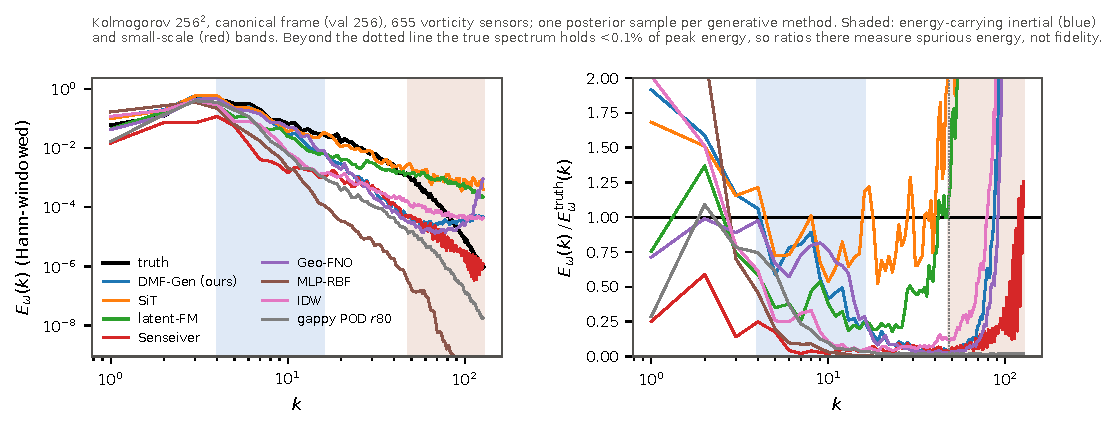
\includegraphics[width=\textwidth]{figures/spectra_kolmogorov.pdf}
\caption{\label{fig:spectra2d}Kolmogorov $256^2$ shell spectra of single
samples on the canonical frame, 655 vorticity sensors, Hann-windowed. Left:
spectra against DNS. Right: ratio to truth. Shaded: the energy-carrying
inertial band (blue) and the small-scale band (red). Beyond the dotted line the
true spectrum holds under 0.1\% of its peak, so ratios there measure energy a
method invented rather than energy it recovered --- which is why we score
fidelity on the shaded bands and report the tail separately.}
\end{figure*}

\begin{figure*}[tbp]
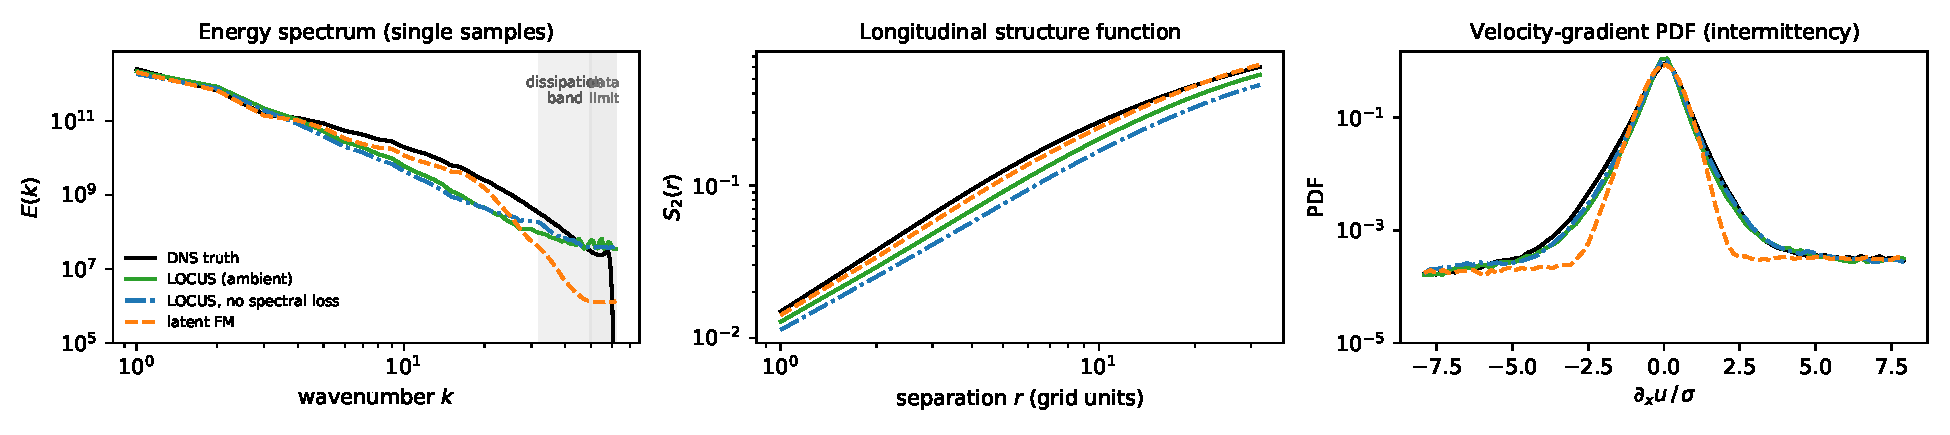
\includegraphics[width=0.9\linewidth]{figures/spectra_stats.pdf}
\caption{\label{fig:spectra}Turbulence statistics of single posterior samples
on the held-out 3D region (4 snapshots, NFE 4, Hann-windowed; ensemble means
are deliberately not shown --- averaging destroys small scales by
construction). Left: shell-averaged energy spectra --- the latent baseline
tracks the DNS through the inertial range then falls away sharply in the
dissipation band (autoencoder floor); the ambient model sits lower in the
inertial range and flattens into a noise plateau at high $k$. Middle:
longitudinal structure functions. Right: velocity-gradient PDFs.}
\end{figure*}

\subsection{Computational cost and scaling}\label{sec:cost}

\begin{figure}[tbp]
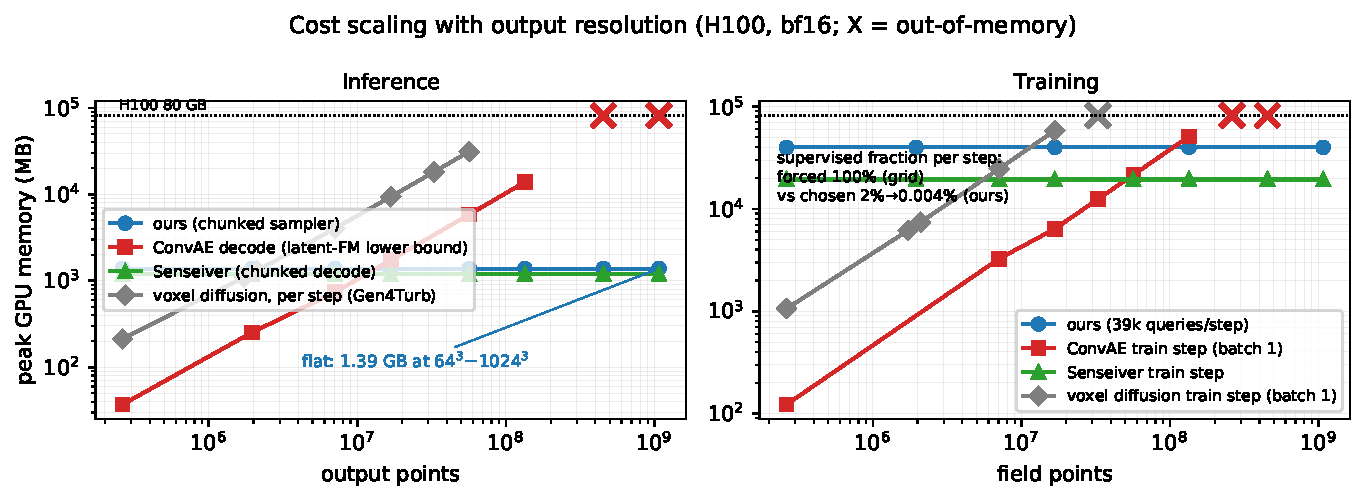
\includegraphics[width=\linewidth]{figures/scaling_cost_mem.pdf}
\caption{\label{fig:scaling}Measured peak memory versus output resolution
(H100, bf16, log--log; OOM markers are measured failures, not
extrapolations) for full-field sampling (left) and training steps (right).
Grid methods (voxel diffusion, convolutional AE) scale cubically and fail at
$320^3$ and $640^3$; point methods (\dmfgen{}, Senseiver) are flat to
$1024^3$ ($10^9$ points). Annotation: fraction of the field supervised per
training step --- 100\% forced for grid methods, a fixed 39k-point budget for
the subsampled point method.}
\end{figure}

Cost separates the fleet along two axes. At the benchmark resolution
(Table~\ref{tab:jhucost}), total training cost to a finished model spans
7--19 GPU-hours across learned methods --- comparable --- but inference
spans five orders of magnitude, from 19\,ms (latent decode) to minutes
(chunked token generation, DPS optimization), and peak training memory spans
3.6--54\,GB. Against resolution (Fig.~\ref{fig:scaling}), the fleet splits
into two families: grid computation (voxel diffusion, convolutional
autoencoders) scales cubically with measured out-of-memory walls at $320^3$
(training, batch 1) and $640^3$, while point computation (attention over
sensors with chunked queries) is flat to $1024^3$ in both training and
inference memory. The honest converse is that grid computation is cheaper
below the crossover (${\sim}240^3$ for inference: a convolutional decode of a
$125^3$ field costs 6\,ms where chunked point evaluation costs seconds). No
family dominates; the benchmark's contribution is that the walls and
crossovers are measured, so a practitioner can place their discretization on
the axis before choosing a method family.

\begin{figure}[tbp]
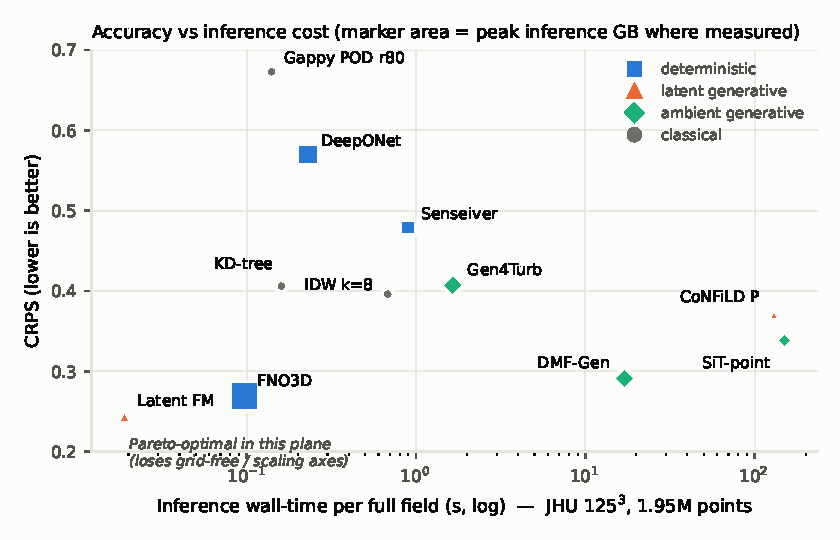
\includegraphics[width=\linewidth]{figures/pareto_cost_accuracy.pdf}
\caption{\label{fig:pareto}Probabilistic accuracy (CRPS, JHU cross-cube,
$n{=}50$) against inference wall-time per full $125^3$ field, marker area
proportional to peak inference memory where measured
(Table~\ref{tab:jhucost}). At the benchmark resolution the latent
flow-matching baseline Pareto-dominates this plane outright --- fastest and
lowest CRPS --- which is precisely why a single cost--accuracy plot is an
insufficient basis for method choice: the axes it cannot show
(Fig.~\ref{fig:capability}; the scaling walls of Fig.~\ref{fig:scaling})
are where the grid-locked methods lose. S3GM is absent from this plane: its
upstream sampler diverges at 3D scale, and its two labelled retuned arms are
reported in Table~\ref{tab:jhu} rather than plotted as if they were the
published method (Sec.~\ref{sec:jhu}).}
\end{figure}

Figure~\ref{fig:pareto} makes the same point from the accuracy side: on the
cost--accuracy plane alone the latent baseline dominates every method
including \dmfgen{}, and the case for ambient point-cloud generation rests
entirely on the axes the plane omits --- resolution scaling and
dissipation-range fidelity, measured here, and geometry-freedom and
operator robustness, which the deferred multiphysics and unstructured-geometry
regimes are designed to measure (Sec.~\ref{sec:discussion}).

\subsection{Why benchmark numbers look worse than the literature's ---
protocol, not architecture}\label{sec:leakage}

Readers who compare our tables and galleries against published
reconstruction papers --- including papers evaluated on the very same
Kolmogorov data\cite{shu2023physics} --- will notice that every method here,
including the strong ones, scores and \emph{looks} worse. We consider this
observation a central result of the benchmark rather than an embarrassment,
because each contribution to the gap is a protocol choice, and we measure
them separately.

\emph{(i) Splits: interpolation vs.\ generalization.} On 617 consecutive DNS
frames, frame-to-frame correlation is 1.00 at unit separation and 0.67 at
separation 100, and a shuffled random-in-time split places every evaluation
frame within one frame of a training frame. Under that split the latent
flow-matching baseline scores 0.14 relative $L_2$; under the spatially
disjoint protocol the same architecture, data, and budget scores 0.56 ---
and the entire fleet shifts by factors of 2--4, unevenly, so leakage does
not merely inflate scores, it \emph{reorders methods}: models with the
capacity to memorize the training trajectory (latent codecs;
sensor-identified frame lookup) gain most. The 2D fleet reproduces the
mechanism: Senseiver reaches 0.17 training loss but 0.91 held-out-trajectory
error on Kolmogorov --- the same memorization that a same-trajectory split
would have rewarded as excellence. The controlled 2D ablation sharpens the
mechanism: the \emph{same} \dmfgen{} checkpoint evaluated on unseen frames
of \emph{seen} trajectories scores 0.483 against 0.487 held-out --- no gain,
because this model never memorized (its train and validation losses track).
We predicted that Senseiver, the fleet's clearest memorizer, would collapse
toward its 0.17 training loss under the same-trajectory split. \emph{It does
not.} Measured on the identical checkpoint and frames, it improves only from
0.913 to 0.873, a 4.4\% gain against \dmfgen{}'s 0.9\% and SiT's 0.6\%. The
ordering of the prediction survives --- the memorizer does gain several times
more than the others --- but the magnitude does not: a leaky \emph{split} is
worth a few percent to anyone here, nowhere near enough to reorder a fleet
whose adjacent gaps are 0.1 or larger. The contrast with the 3D numbers above
is not a contradiction but a dose--response: the 3D shuffle places an
evaluation frame \emph{adjacent} to a training frame in the same trajectory,
whereas this 2D arm holds out frames of a seen trajectory that are already
four DNS steps apart, and the residual correlation at that separation is
simply too small to exploit. Leakage severity is a property of how close the
nearest training frame is, not of whether the word ``split'' was used.

That result relocates the blame. Of the total gap to literature-style
reporting, the sensor \emph{layout} carries almost all of it: moving from
scattered to uniform-lattice sensing takes \dmfgen{} from 0.487 to 0.367, a
25\% reduction, and combining uniform sensing with the leaky split adds
essentially nothing beyond it (0.364). The interpolation floor moves the same
way (IDW 0.546 scattered, 0.452 uniform), which is the tell that this is a
property of the measurement geometry rather than of any model: uniformly
spaced sensors bound the worst-case distance to data, and reconstruction error
at 1\% sparsity is dominated by that distance. A benchmark that adopts uniform
sensing because it is convenient therefore reports a systematically easier
problem, and no amount of split hygiene compensates for it. Our headline claim
is consequently narrower than we first drew it: \emph{protocol, not
architecture} remains right, but within protocol it is the sensing layout that
dominates, and the split matters mainly as a correctness requirement rather
than as a large numerical effect.
\todo{PROVENANCE, blocking: the 3D pair quoted in this paragraph (0.14
shuffled / 0.56 honest) cannot be sourced from the artifacts on the current
host. The archived pre-fix evaluations were never transferred, and no latent-FM
JHU evaluation in the present tree scores either value --- the three that exist
all aggregate to 0.468--0.469, which is the number Table~\ref{tab:jhu} reports.
The 0.56 in that table's latent-FM row is its \emph{coverage}, not its
rel-$L_2$, so the honest half of the pair as written contradicts our own table.
Two things are needed and neither should be guessed: (a) the archived
shuffled-split JSONs, from which the 3-method table and the ``factors of 2--4''
range would be assembled, and (b) confirmation of which run the honest half
refers to. Until (a) lands, the quantitative 3D leakage claim in this paragraph
and in the introduction must be either re-sourced or narrowed to the 2D
protocol ablation below, which IS measured here. Do not simply substitute 0.469
for 0.56: that would mix a current run into a pair whose other half comes from
the archive.}

\emph{(ii) What ``1\% sparsity'' means.} Much of the visually striking
literature conditions on uniformly downsampled coarse grids --- every cell
of a coarse lattice, i.e.\ band-limited full-field information with bounded
gaps --- or adds physics guidance (PDE-residual or forcing terms at sampling
time\cite{shu2023physics,huang2024diffusionpde}). Our protocol uses randomly
scattered points and purely data-driven conditioning: the same nominal
percentage carries far less information and admits large sensor-free
regions. Measured on Kolmogorov with the same checkpoint and frames,
rearranging the 655 scattered sensors onto a uniform $25{\times}26$ lattice
improves \dmfgen{} from 0.487 to 0.367 relative $L_2$ (CRPS $0.235{\to}
0.171$) and IDW from 0.546 to 0.452 --- a 25\% accuracy difference from
sensor \emph{layout} alone, before any change of model or split.

\emph{(iii) What is shown.} Publication figures typically display ensemble
means or favorable frames; we display single posterior samples on fixed,
pre-registered frames (our gallery frame runs $0.65$--$0.96$ across the
fleet against $0.39$--$0.50$ fifty-frame averages), because single-sample
behavior is what the physics metrics score. Ensemble size interacts with the
same point: $K{=}8$ coverage understates calibration
(Sec.~\ref{sec:metrics}), and ensemble means visually erase exactly the
small scales the spectra measure.

\emph{(iv) Matched budgets.} Every model trains at a matched
${\sim}50$k-step budget with disclosed tuning asymmetry, not to per-method
convergence. Fairness costs polish; the cost table prices it.

The synthesis we intend a reader to take away: \emph{apparent reconstruction
quality in this literature is substantially a property of evaluation
protocol, and only secondarily of architecture.} A benchmark that fixes the
protocol first makes the remaining --- genuine --- architectural differences
measurable.

\section{Discussion}\label{sec:discussion}

\paragraph{Which method should a practitioner use?} The benchmark's answer is
conditional, and that is the point. If sensing is dense relative to the
flow's intrinsic dimension (laminar, periodic regimes) use interpolation or
gappy POD; nothing learned earns its training cost there --- on the cylinder
the rank-20 POD floor beats all seven learned methods, and the margin over
the best of them is statistically resolved (Sec.~\ref{sec:cylinder}). On observed channels of turbulence at
${\sim}$1\% density, training-free interpolation remains competitive with the
best learned methods --- the case for learning begins where the problem is
ill-posed: unobserved channels and sparser sensing in this suite, and, beyond
it, corrupted or surface-confined operators. There, deterministic learners
are structurally limited to conditional means; among generative routes,
latent compression buys inference speed and global field structure at a
measured dissipation-range floor, while ambient point-cloud generation buys
small-scale fidelity at higher inference cost, with geometry-freedom and
operator amortization as the structural advantages the deferred regimes are
designed to test. If the discretization exceeds ${\sim}300^3$, grid families
exit on measured walls; if it lives on a body-fitted or unstructured mesh,
they exit on interface grounds, as the cylinder's grid export already
illustrates. Uncertainty from any
current method must be recalibrated before operational use, and the benchmark
ships the wrapper.

\paragraph{Limitations.} All three regimes are simulation data on
canonical flows, and all three are Cartesian or near-Cartesian --- two
periodic Cartesian grids and one body-fitted O-grid around a circular
cylinder --- so the present suite measures neither measurement realism nor
geometric generality: the multiphysics regime with realistic corrupted
measurement operators (wildfire LES) and the unstructured, case-varying
geometry regime with surface-only sensing (transonic wing family) are
deferred to a follow-up paper, and the corresponding claims about operator
robustness and geometry-freedom are stated here only as structural
properties of the interfaces, not as measured results. All learned rows
train per-regime (no pretraining across flows); the suite contains no
experimental data --- particle-image-velocimetry or
pressure-sensitive-paint regimes with real sensor noise are the natural
next addition; single-snapshot reconstruction
ignores temporal information that assimilation exploits; the cost accounting
is single-GPU (H100) and does not probe multi-GPU scaling; the tuning-budget
asymmetry of Sec.~\ref{sec:fairness} item (v) is disclosed but not
eliminated; and training-seed variance is measured for the 2D fleets
(Sec.~\ref{sec:kolmogorov}) but not for the 3D one, where a single replicate
costs more than the rest of the suite combined.

\section{Conclusion}\label{sec:conclusion}

\benchname{} turns sparse-sensor flow reconstruction from a collection of
incompatible per-paper evaluations into a measured landscape: three regimes,
twelve-plus audited methods, proper probabilistic scoring, physics metrics
with their estimator pitfalls documented, matched cost accounting, and
leakage-controlled splits with the distortion of the dominant protocol
quantified. The findings that outlive any single table: method ranking is
regime-dependent and no method wins twice; the classical floor is sometimes
unbeaten, and which classical method constitutes it changes with the regime;
unobserved channels are near-unidentifiable in 3D turbulence yet recoverable
on the cylinder by a linear basis, so identifiability is a property of the
flow rather than of the method; mean-field error alone misranks generative
methods, and on Kolmogorov it reverses the ranking between accuracy and CRPS
across whole method families; nearly every scored ensemble is under-dispersed
and post-hoc recalibration repairs stated coverage; and the computational axis
separates grid from point families at measured walls. The datasets, splits,
sensor manifests, configurations, audit notes, and evaluation driver are
released for extension --- the leaderboard is meant to be beaten.

\begin{acknowledgments}
\todo{funding/compute acknowledgments; DMF-Gen authors; JHTDB dataset
providers.}
\end{acknowledgments}

\section*{Data availability}
The benchmark artifact --- datasets or regeneration recipes (JHTDB cutout
coordinates and download scripts, OpenFOAM case definitions, converter
scripts), split manifests, seeded sensor draws, per-method configurations,
audit notes, and the evaluation driver --- will be released on acceptance.
\todo{Zenodo/HF DOI; confirm JHTDB redistribution terms (fallback: recipe +
coordinates); needs sign-off before anything goes public.}

\bibliography{references,refs_extra}

\end{document}
